\documentclass[a4paper,11pt]{report}

\usepackage{fullpage}
\usepackage[utf8]{inputenc}
\usepackage{t1enc}
\usepackage[spanish]{babel}
\usepackage[pdftex,usenames,dvipsnames]{color}
\usepackage[pdftex]{graphicx}
\usepackage{enumerate}
\usepackage{url}
\usepackage{amsmath}
\usepackage{amsfonts}
\usepackage{amssymb}
\usepackage{comment}
\usepackage{lastpage}
\usepackage[table]{xcolor}
\usepackage[small,bf]{caption}
\usepackage{float}
\usepackage{subfig}
\usepackage{bm}
\usepackage{fancyhdr}
\usepackage{times}
\usepackage{titlesec}
\usepackage{csquotes}
\usepackage[backend=bibtex,sorting=none]{biblatex}
\usepackage{titling}
% \usepackage{algorithmicx}
\usepackage{algpseudocode}
\usepackage{algorithm}
\usepackage{letltxmacro}
\usepackage[margin=1cm]{caption}
\usepackage{setspace}
\usepackage[titletoc]{appendix}

%%%%% BEGIN ALGPSEUDOCODE STUFF %%%%%%
\algdef{SxnE}[FOREACH]{ForEach}{EndFor}[1]{\algorithmicfor\ #1\ \algorithmicdo}
% LEAVES BLANK LINE AT END \algblockdefx[FOREACH]{ForEach}{EndFor}{\textbf{for each }}{}
\algdef{SxnE}[FOR]{For}{EndFor}[1]{\algorithmicfor\ #1\ \algorithmicdo}
\algdef{SxnE}[WHILE]{While}{EndWhile}[1]{\algorithmicwhile\ #1\ \algorithmicdo}
\algdef{SxnE}[IF]{If}{EndIf}[1]{\algorithmicif\ #1\ \algorithmicthen}
\algdef{cxnE}{IF}{Else}{EndIf}

\renewcommand{\algorithmicrequire}{\textbf{Input:}}
\renewcommand{\algorithmicensure}{\textbf{Output:}}
\algnewcommand\algorithmicauxiliary{\textbf{Auxiliary:}}
\algnewcommand\Auxiliary{\item[\algorithmicauxiliary]}

\DefineBibliographyStrings{spanish}{andothers = {et\addabbrvspace al\adddot}}
\renewbibmacro{in:}{}

\floatname{algorithm}{Algoritmo}

\DeclareMathOperator*{\argmin}{arg\,min}
\addbibresource{references}
\DeclareFieldFormat[inbook]{citetitle}{#1}

\newcommand{\norm}[1]{\left\lVert#1\right\rVert}

\renewcommand\appendixtocname{Anexo}

% \titleformat{\section}{\small\center\bfseries}{\thesection.}{0.5em}{\normalsize\uppercase}
% \titleformat{\subsection}{\small\center\bfseries}{}{0.5em}{\small\uppercase}

\def\customabstract{\vspace{.5em}
    {\Large\center{\textbf{RESUMEN}} \\[0.5em] \relax
    }}
\def\endcustomabstract{\par}

\def\keywords{\vspace{.5em}
    {\textit{Palabras clave: }
    }}
\def\endkeywords{\par}

% TITLE Configuration
% \setlength{\droptitle}{-25pt}
\pretitle{\begin{center}\Huge\begin{rmfamily}}
\posttitle{\par\end{rmfamily}\end{center}\vskip 0.5em}
\preauthor{\begin{center}
        \large \lineskip 0.5em%
\begin{tabular}[t]{c}}
\postauthor{\end{tabular}\normalsize
    \\[1em] Instituto Tecnológico de Buenos Aires
    \\[1em] Proyecto Final Ingeniería en Informática
    \\[1em] Director: Dra. Juliana Gambini
\par\end{center}}
\predate{\begin{center}\small}
\postdate{\par\end{center}}

% Headers
% \addtolength{\voffset}{-40pt}
% \addtolength{\textheight}{80pt}
\renewcommand{\headrulewidth}{0pt}

\fancyhead{}
\fancyfoot{}
\lhead{\small } % No publicado
\rhead{\small }
\fancyfoot[C]{\small Copyright \copyright 2013 ITBA}
\fancyfoot[R]{\thepage}
\renewcommand{\footrulewidth}{0.4pt}

\fancypagestyle{plain}{
  \fancyhf{}% Clear header and footer
  \fancyhead{}
  \fancyfoot{}
  \lhead{\small } % No publicado
  \rhead{\small }
  \fancyfoot[C]{\small Copyright \copyright 2013 ITBA}
  \fancyfoot[R]{\thepage}
  \renewcommand{\footrulewidth}{0.4pt}
}

% Next 4 lines allow for parts with independet sections counters
% and correct referencing between parts

% Metadata
\title{Interpretación y Análisis Automático de Imágenes de Partidos de Fútbol}
\date{1 de agosto de 2014}
\author{Civile, Juan Pablo \and Crespo, Álvaro \and Ordano, Esteban }


\begin{document}
\pagestyle{fancy}
\maketitle

\addvspace{3em}
\begin{customabstract}
\begin{doublespace}
El seguimiento de objetos en una secuencia de imágenes (video) puede ser
aplicado eventos deportivos. En esta aplicación el objetivo es detectar y
seguir la posición de los jugadores y la pelota a medida
que se desarrolla el juego, obteniendo información útil para distintas
aplicaciones, como puede ser brindar soporte informático para los árbitros
(detección automática de pases, goles, posiciones adelantadas, etc...),
colaborar con el cuerpo técnico en el entrenamiento de los jugadores,
el análisis y el estudio de las tácticas de un contricante, entre otros.

En el presente trabajo se propone un método de seguimiento de jugadores que
puede utilizarse para cumplir algunos de los objetivos del problema, se
analizan las dificultades de realizar el seguimiento de jugadores en tiempo
real con reducida o nula supervición humana a partir de una sola fuente de
video que consiste en una cámara de alta resolución (HD) fija capaz de
encuadrar todo el campo de juego.

En base al análisis de dificultades, se selecciona una técnica de seguimiento
y se detalla un algoritmo construido sobre ésta para la tarea específica de
detección y seguimiento de jugadores en partidos de fútbol. Se presentan los
resultados de aplicar este algoritmo, se comparan con otro método existente en
la literatura y se explicita qué información se podría proveer para el análisis
de imágenes de partidos de fútbol.
\end{doublespace}
\end{customabstract}

\tableofcontents

\pagestyle{fancy}
\chapter*{Introducción}
\addcontentsline{toc}{chapter}{Introducción}

Dentro del campo del análisis y tratamiento de imágenes un problema que se
estudia es el del reconocimiento y seguimiento de objetos en secuencias de
imágenes. Identificar correctamente un objeto en un video es útil para un
amplio rango de aplicaciones, como ser aplicaciones médicas (dónde se ofrece
soporte para diagnósticos y cirugías), la industria cinematográfica (captura de
movimiento, \textit{post-producción}), vigilancia automática con cámaras y
juegos interactivos. También tiene una gran influencia en el reconocimiento de
caras y el seguimiento de ojos, técnicas que actualmente son muy utilizadas y
estudiadas, y que tienen una gran potencialidad para ser implementadas en
nuevos campos.

En el ámbito deportivo existen muchas aplicaciones para el seguimiento de
objetos. Puede resultar útil para validar o reemplazar las decisiones de los
jueces o árbitros del partido, permitir a deportistas de alto rendimiento
analizar y mejorar sus movimientos, ayudar a los entrenadores a decidir
estrategias y evaluar a los deportistas, otorgar estadísticas a fanáticos del
juego, entre otras aplicaciones.

El seguimiento de objetos en video consiste en detectar objetos de interés en
el primer cuadro de un video y seguirlo a lo largo de toda la secuencia de
imágenes. Existen varios tipos de métodos que se pueden utilizar para llevar
a cabo esta tarea, los cuales se diferencian en la forma en que representan
a los objetos a seguir o en la manera en que localizan a cada objeto en una
imagen de la secuencia. Por ejemplo, existen métodos de seguimiento que
representan a los objetos de interés por marcas en la imagen y realizan el
seguimiento de las mismas, asociando las marcas entre dos cuadros consecutivos.
El método utilizado en este trabajo representa los objetos de interés por
medio de curvas que representan los contornos de los objetos a seguir y
realiza el seguimiento modificando estas curvas cuadro a cuadro,
intercambiando puntos entre dos listas de píxeles vecinos.

En este trabajo se estudia el problema de realizar el seguimiento de todos los
jugadores de un partido de fútbol, utilizando una única cámara, con su posición
fija y cuyo campo visual abarca todo el campo de juego. Se busca que el seguimiento sea en
tiempo real, es decir, que el procesamiento sea lo suficientemente rápido para
que se vean los resultados mientras se ejecuta el video. Teniendo en cuenta la posición
a través del tiempo, se puede informar la velocidad de un jugador en un
determinado momento, distancia recorrida, zonas más frecuentadas por el
jugador, entre otros.

Se plantea el uso de una técnica de seguimiento existente, basada en
\textit{contornos activos}, para el seguimiento en tiempo real de los
jugadores con una única computadora. Esta técnica determina el contorno de
un objeto dentro del video y a medida que el objeto se mueve el contorno se
adapta tomando decisiones basadas en variaciones de color de los píxeles de los
objetos de interés y de sus alrededores. Se investigan alternativas para
mejorar el seguimiento específicas a las características de un video de fútbol,
como ser la morfología de los objetos a seguir, como por ejemplo, se acota con
un rectángulo más alto que ancho el tamaño máximo del contorno de un jugador,
entre otros.

El trabajo se encuentra compuesto de la siguiente manera: en el Capítulo
\ref{chap-state} se describe el estado del arte actual en el área de
seguimiento de objetos, y en particular se examinan soluciones aplicadas al
análisis automático de eventos deportivos. En el Capítulo
\ref{chap-problems} se detalla el problema a solucionar y se discuten las
dificultades del seguimiento automático. En el Capítulo \ref{chap-ac} se
resume el márco teórico y el funcionamiento del algoritmo de seguimiento
utilizado. El contenido del Capítulo
\ref{chap-solution} describe la solución planteada, estrategias que otorgaron
mejores resultados, así como variaciones que fueron implementadas y
posteriormente descartadas por no mejorar los resultados. El Capítulo
\ref{chap-results} muestra los resultados obtenidos al ejecutar el algoritmo en
videos filmados en partidos de fútbol profesional de clubes argentinos, y
ofrece una comparación de la performance de la solución propuesta con otro
algoritmo de seguimiento existente que no fue optimizado
para seguimiento de jugadores de fútbol. Para finalizar, en el Capítulo
\ref{chap-conclusion} se presentan las conclusiones del trabajo.

\newpage

\chapter{Estado del arte}
\label{chap-state}

\section{Algoritmos de seguimiento}

\label{sec:tracking}

A continuación se describen los algoritmos de tres familias dentro de la rama
de análisis de imágenes para seguimiento de objetos.

\subsection{Predictores Lineales}

Un \textit{Predictor Lineal} es una función que toma los valores de una serie
de variables aleatorias y predice el valor de una variable dependiente.  La
función tiene la forma $f(x_1, ..., x_n) = \beta_0 + \beta_1 x_1 + \dots +
\beta_n x_n$, donde $x_i$ es una variable aleatoria y $\beta_i$ una constante.
Se dice que el predictor es lineal debido a la condición $\beta_i \in \mathbb{R}$
\footnote{Cualquier $x_i$ no lineal, puede expresarse como $x'_i = g(x_i)$ y tratarse como lineal}.

En los artículos \cite{alp, original-linear-predictors} los autores utilizan
predictores para hacer seguimiento de objetos en video.  El objetivo es
relacionar el cambio de valor de varios píxeles cuadro a cuadro con el
movimiento del objeto entre dichos cuadros.  Para soportar cualquier clase de
movimiento, este se representa mediante una homografía (ver
\cite{homography-estimation}), $H \in R^{3\times3}$.

Los predictores se representan mediante una matriz $A \in \mathbb{R}^{9xn}$
donde cada fila representa una función de predicción.  De dos cuadros
consecutivos se obtiene el vector de cambios de los valores de píxeles $X = (x_1,
\dots, x_n)$ y se computa:

\begin{eqnarray*}
    AX &=& B \\
    B &=& (h_{1,1}, h_{1,2}, h_{1,3}, h_{2,1}, h_{2,2}, h_{2,3}, h_{3,1}, h_{3,2}, h_{3,3})
\end{eqnarray*}

Donde $B$ contiene los valores de la homografía $H$ de movimiento entre los cuadros.

\subsubsection{Cálculo de los predictores}
Para obtener la relación $A$ se utiliza un paso inicial de entrenamiento.
Primero se determina la posición del objeto en un cuadro de manera supervisada.
Una vez conocida la posición, se toman $n$ muestras aleatorias del valor de
píxeles en ese cuadro.

Luego se crean $m$ perturbaciones de la posición del objeto, y se computa la
homografía $H_i$ (para $i = 1, 2, \dots m$) que representa la perturbación.
Se denomina $B_i$ al vector que representa cada homografía. Además, se toman
muestras de valores de píxeles ($X_i$) con sus posiciones alteradas por la
homografía $H_i$. Se plantea:

\begin{equation}
    A \left( X_1 \lvert \dots \lvert X_m \right) = \left( B_1 \lvert \dots \lvert B_m \right)
\end{equation}
El cual es un sistema de ecuaciones lineales que puede ser resuelto de manera sencilla.

\subsubsection{Mejoras}

Para mejorar la efectividad de los algoritmos, se calculan varios predictores y se disponen en capas.
Cada capa se construye para buscar cambios de posición cada vez más finos o pequeños.
Es decir, la primer capa busca cambios bruscos y la última pequeños cambios.

\citeauthor*{alp} (ver \cite{alp}) introducen una nueva técnica para manejo de oclusiones
parciales de manera eficiente. Para esto se divide el objeto en pequeñas
secciones cuadradas, llamadas \textit{templates}, y se computa la matriz $A$ de
la siguiente manera:

\begin{eqnarray*}
    Y &=& \left( B_1 \lvert \dots \lvert B_m \right) \\
    H &=& \left( X_1 \lvert \dots \lvert X_m \right) \\
    A &=& Y H^T(HH^T)^{-1}
\end{eqnarray*}

Esto permite actualizar $A$
rápidamente para remover y agregar \textit{templates}. Es decir, permite ignorar
secciones ocultas del objeto hasta que éstas vuelven a ser visibles.

\subsection{Aprendizaje Local}
% Local learning

El aprendizaje local es otra técnica que permite resolver el problema del
seguimiento de objetos en secuencias de imágenes, que ha sido también un tema
de investigación en el área del aprendizaje automático (ver
\cite{local-learning-machine-learning}) y usado principalmente en la
clasificación de imágenes, recuperación y reconocimiento de objetos.

A diferencia del aprendizaje global, que entrena un modelo basado en
todos los datos de entrenamiento, en \textit{local learning} se consideran
varios modelos locales, cada uno extraído de solamente un subconjunto de los
datos de entrenamiento. Este tipo de enfoque enfatiza la idea de que un modelo
local puede caracterizar mejor las propiedades intrínsecas y discriminativas de
su correspondiente subconjunto de datos, que un modelo global para el conjunto
completo de datos. De esto se desprende que utilizar múltiples modelos locales
puede ofrecer mejores resultados cuando los datos están distribuidos de manera
complicada o poco clara.

Si bien se puede pensar al seguimiento de objetos como una tarea de clasificación binaria
que apunta a separar el objeto del resto de la imagen o fondo, en realidad, el principal
problema reside en relacionar las apariciones del objeto entre dos cuadros
consecutivos. Esto se logra mediante una función de distancia que
establece el grado la similaridad entre los puntos característicos \footnote{Los puntos
  característicos son puntos que se diferencian del resto por poseer o mostrar
ciertas características específicas y representativas. En el caso del
seguimiento de objetos, son los puntos que mejor representan las
características del objeto, y que tienen mayor resistencia a variar con los
diferentes cambios de escala, rotación, iluminación, etc...} de cada cuadro.

La elección de la medida de distancia es de suma importancia. A modo de
ejemplo, la distancia Euclideana puede llevar a algoritmos de seguimiento
inestables a la hora de diferenciar el objeto del fondo de la imagen. Por lo
tanto, se requiere una mejor y más compleja medida de distancia. Esta es la
idea princial que proponen Li y Lu (ver \cite{local-learning}).

La función de distancia que usan es una combinación lineal de distancias
elementales, como se presenta en \cite{malisiewicz-cvpr08}. Definen a la
función de distancia entre dos puntos característicos, a los que llaman
\textit{ejemplares}, $e$ y $z$ como:

\begin{equation}
    \label{eq:distance-exemplar}
    D_{e}(z) = w_{e} \cdot d_{ez}
\end{equation}

donde $w_{e}$ es el vector de pesos de $e$, y $d_{ez}$ es el vector de
distancia n-dimensional entre $e$ y $z$, cuya n-ésima componente es la
distancia $L_{2}$ entre la característica n-ésima de $e$ y $z$. Cabe destacar
que la función del vector de pesos, $w_{e}$, es asignar una importancia relativa a
la distancia de cada componente de $d_{ez}$. De esta forma, se ponderan las distancias
entra ciertas características por sobre otras.

Cada ejemplar está también asociado con un vector binario $B_{e}$, cuyos elementos
no nulos implican que los ejemplares correspondientes son similares a $e$. La
longitud de $B_{e}$ es igual al número de ejemplares con el mismo rótulo de $e$
\footnote{Se dice que un conjunto de ejemplares tiene un mismo rótulo si pertenecen a un mismo objeto. En el caso de seguimiento de objetos
más sencillo, exitirían 2 objetos: el objeto a seguir, y el fondo}.
Asumiendo que el aprendizaje de cada una de las funciones de distancia es
independiente del resto, se puede aprender $w_{e}$ y $B_{e}$, en un problema
de aprendizaje formulado de la siguiente manera:

\begin{equation}
    \label{eq:learning-problem}
    f_{1}(w,B) = \sum_{i \in C} B_{i}L(-w \cdot d_{i}) + \sum_{i\notin C}L(w \cdot d_{i})
\end{equation}
\begin{equation}
    {w^{*}, B^{*} = \argmin_{w,b} f_{1} (w,b) }
\end{equation}
\begin{equation}
   w \geq 0, B_{i} \in {0,1}, \sum_{i} B_{i} = M
\end{equation}

Nótese que se descarta el subíndice $e$ para tener una mayor claridad. El
conjunto $C$ es el conjunto de todos los ejemplares con el mismo rótulo que $e$
y $M$ es el mínimo número de ejemplares similares a $e$ (predefinido). La
función $L$ puede ser cualquier función de costo o pérdida \footnote{Una
función de pérdida o función de costo es simplemente una función que mapea un
evento o los valores de una o más variables a un número real que representa
algún ``costo'' asociado al evento.} , estrictamente positiva. El vector de
pesos $w$ se requiere que sea positivo para asegurar que una mayor distancia
elemental (entre alguna de las características) no pueda nunca llevar a una
menor distancia total, lo que implicaría una mayor similaridad.

Previo al seguimiento se deben especificar manualmente algunos parámetros iniciales,
como ser: punto central, ancho, altura y rotación del objeto. En el proceso de
entrenamiento, se aplica un Análisis de la Componente Principal
\footnote{El Análisis de la Componente Principal, es una técnica utilizada para reducir la dimensionalidad de un conjunto de datos.
Sirve para hallar las causas de la variabilidad de los datos y ordenarlas por importancia.
Técnicamente, busca la proyección según la cual los datos queden mejor representados en términos de cuadrados mínimos. Involucra el cálculo de la descomposición en
autovalores de la matriz de covarianza, normalmente tras centrar los datos en la media de cada atributo.}
de forma incremental en los primeros $F$ cuadros. En su trabajo, Li y Lu usan
$F = 5$ (ver \cite{local-learning}).

Los mejores resultados se seleccionan como muestras de entrenamiento positivas, mientras que
los peores resultados, se toman como muestras negativas. Se obtienen las características
RGB y LBP, como se presentan en \cite{tracking-bag-of-features}, de todas las muestras,
tanto positivas como negativas. Para cada muestra de entrenamiento, se calculan las
distancias elementales RGB y LBP con respecto a todas las restantes muestras.

Para obtener el vector de pesos óptimo, $w^{*}$, se calcula iterativamente $B$,
en función de $w$, y $w$ en función de $B$, asegurando que el valor de $f_{1}$ nunca
crezca, para encontrar un mínimo local. Este proceso iterativo se puede modelar de la
siguiente forma:

\begin{equation}
   \label{eq:local-learning-B-k}
   B^{k} = \argmin_{B} \sum_{i \in C} B_{i}L(-w^{k} \cdot d_{i})
\end{equation}
\begin{equation}
    \label{eq:local-learning-w-k}
    w^{k+1} = \argmin_{w} \sum_{i:B_{i}^{k}=1} L(-w \cdot d_{i}) + \sum_{i\notin C}L(w \cdot d_{i})
\end{equation}

Dado un $w^{k}$, que inicialmente podría ser aleatorio, se minimiza la ecuación
\ref{eq:local-learning-B-k} fijando $B_{i} = 1$ para los $M$ valores más
pequeños de $L(-w \cdot d_{i})$ y $0$ para el resto. Dado $B^{k}$, se puede
obtener fácilmente $w^{k}$, resolviendo la ecuación \ref{eq:local-learning-w-k}.
El aprendizaje termina cuando $B^{k+1}=B^{k}$.\\

En el proceso de seguimiento, para cada cuadro nuevo, se determinan cuáles son los candidatos
a ser ejemplares. En el área del aprendizaje automático, siempre se seleccionan
candidatos para luego verificar si cumplen las condiciones requeridas. En este
caso, se quiere ver si los candidatos cumplen con las condiciones necesarias
para ser puntos característicos. Para ello, se seleccionan
aleatoriamente aplicando un filtro de partículas
\footnote{El filtro de partículas es un método empleado para estimar el estado
  de un sistema que cambia a lo largo del tiempo. Más concretamente es un
  método de Montecarlo(secuencial). Se compone de un conjunto de muestras (las
  partículas) y valores, o pesos, asociados a cada una de esas muestras.
  Las partículas son estados posibles del proceso, que se pueden representar
  como puntos en el espacio de estados de dicho proceso.}
sobre el resultado del cuadro anterior. Luego, se extraen las características
RGB y LBP como muestras de testeo. Después de calcular las distancias
elementales entre las muestras de testeo y de entrenamiento, se forma una
matriz de distancia, $D \in R^{N_{test} \times N_{train}}$ a través de las
funciones de distancia entrenadas. Es decir, el elemento $(i,j)$ de la matriz
$D$, contiene la distancia entre la muestra de testeo $i$, y la muestra de
entrenamiento $j$.

Finalmente, se utiliza la matriz $D$ para localizar al objeto como sigue:

\begin{equation}
    T = \argmin_{t} c \sum_{i} D_{i}(t) + (1 - c) \sum_{j} D_{j}(t)
\end{equation}

\begin{equation}
    \forall i \in \{i : i \in S^{+}, D_{i}(t) \leq Thr_{D} \}
\end{equation}
\begin{equation}
    \forall j \in \{j : j \in S^{+}, D_{j}(t) > Thr_{D} \}
\end{equation}

Donde $t$ es un candidato y $T$ es el objeto. $S^{+}$ es el
conjunto de muestras de entrenamiento positivas. La idea consiste en
que las muestras cuyas distancias sean menor que el umbral $Thr_{D}$
contribuyan más a localizar el objeto, entonces la constante $c$ debería tener
un valor acorde, $c > 0.5$. Los autores Li y Lu utilizaron $c = 0.7$ (ver
\cite{local-learning}).

El algoritmo de seguimiento se complementa con una idea más, que
contribuye a atacar el problema de los cambios de poses y las oclusiones.
Para esto es necesario actualizar el modelo que se tiene para
que efectivamente pueda manejar estas dificultades.
Haciendo uso del umbral de distancia $Thr_{D}$ para prevenir
malas actualizaciones, se realizan correciones al modelo,
en este caso, las funciones de distancia. Esto es, una distancia
menor a $Thr_{D}$ indica que el candidato pertenece a la misma clase,
mientras que una distancia mayor indica lo contrario. Utilizando
la ecuación \ref{eq:learning-model-update-1}, se agregan candidatos,
como muestras positivas de entrenamiento y cada 5 cuadros,
se utiliza el conjunto actualizado de entrenamiento para
reentrenar todas las funciones de distancia.

\begin{equation}
    \label{eq:learning-model-update-1}
    t_{label} = \left\{
                \begin{array}{l l}
                    1, & D_{S^{+}}(t) \leq Tht_{D}\\
                    0, & D_{S^{+}}(t) >  Tht_{D}
                \end{array} \right.
\end{equation}

\begin{equation}
    \label{eq:learning-model-update-2}
    D_{S^{+}}(t) = \dfrac{1}{N_{S^{+}}} \sum_{i \in S^{+}} D_{i}(t)
\end{equation}

En la ecuación \ref{eq:learning-model-update-2}, $N_{S^{+}}$ es el
número de muestras positivas de entrenamiento y $D_{S^{+}}(t)$
es el promedio de distancia del candidato $t$ a las muestras
de entrenamiento positivas.

\subsection{Basado en Grafos}
% IFTrace

El algoritmo conocido como \textit{IFTrace} (ver \cite{IFTrace}) tiene como objetivo
seguir un objeto en una secuencia de imágenes. Este algoritmo realiza algunas
asunciones sobre el objeto a seguir:

\begin{itemize}
    \item consiste de una o más regiones conexas,
    \item tiene un borde bien definido
    \item sus propiedades intrínsecas pueden variar con el tiempo.
\end{itemize}

Los objetos a seguir son inicialmente marcados de forma interactiva por el
usuario en el primer cuadro, y luego se seleccionan automáticamente varios
marcadores en el interior y los alrededores del objeto. Estos marcadores se
localizan en el siguiente cuadro utilizando en forma conjunta el algoritmo de
seguimiento de características KLT (ver \cite{KLT}) y extrapolación de
movimiento. Los bordes del objeto son entonces identificados a partir de estos
marcadores por la IFT, \textit{Image Foresting Transform} (ver \cite{IFT}).
Otra característica central del algoritmo es el operador de detección de borde
que se adapta gradualmente a cambios en el color y la textura del objeto.

El método IFT trata a la imagen como un grafo, en el cual los píxeles son los
nodos, y estos están conectados mediantes aristas si son adyacentes y tiene un
peso o costo. Este costo debe ser una medida de la probabilidad de que los
puntos estén separados por el borde del objeto de interés. En problemas
sencillos puede ser tan simple como el valor absoluto de la diferencia de color
entre los píxeles. El método combina el gradiente del color con el gradiente de
una función de clasificación difusa (\textit{fuzzy matching}), que consiste en
cuantificar la similitud entre el píxel y el conjunto de píxeles del objeto
segmentado en el frame anterior.

La IFT encuentra caminos de costo mínimo desde los marcadores, tanto internos
como externos, a cada píxel de la imagen. Los píxeles son agrupados en
particiones, que resultan ser árboles de camino óptimo disjuntos,
\footnote{Dado un grafo simple, no dirigido y conexo G, un árbol de camino
  óptimo, o árbol de camino más corto, es un árbol recubridor de $G$, tal que
  la distancia o costo del camino desde la raíz $v$ a cualquier otro vértice
$u$ es la distancia de camino mínima de $v$ a $u$ en $G$.} donde cada árbol
tiene a uno de los marcadores como raíz. La proyección del objeto es entonces
tomada como la unión de los árboles cuyas raíces son marcadores internos.

\subsubsection{El algoritmo IFTrace}
\begin{algorithm}
    \caption{IFTrace}
    \label{alg:IFTrace-algorithm1-IFTrace}
    \begin{algorithmic}
        \Require\hspace{\algorithmicindent}\hspace{\algorithmicindent}Video I : D x \{1..$n_{f}$\} $\to V$
        \State\hspace{\algorithmicindent}\hspace{\algorithmicindent}\hspace{\algorithmicindent}\hspace{0.3cm}donde D = \{1..$n_{x}$\} x \{1..$n_{y}$\}
        \State\hspace{\algorithmicindent}\hspace{\algorithmicindent}\hspace{\algorithmicindent}\hspace{0.3cm}Mascara Binaria $O^{(1)}$ : D $\to$ \{0,1\}

        \Ensure \hspace{\algorithmicindent}\hspace{0.23cm} Mascaras Binarias $O^{(t)}$ : D $\to$ \{0,1\} para $t \in $ \{2..$n_f$\}
        \State

        \For{$t = 2,3, ..., n_f$}
            \State $(R^{(t-1)}_{o}$,$R^{(t-1)}_{x}) \gets $  SelectMarkers($I^{(t-1)}$,$O^{(t-1)}$)
            \State $(S^{(t)}_{o}$,$S^{(t)}_{x}) \gets$  TrackMarkers($R^{(t-1)}_{o}$,$R^{(t-1)}_{x}$,$I^{(t-1)}$,$I^{(t)}$)
            \If{$S^{(t)}_{o}$ $\neq \emptyset$}
                \State $O^{(t)} \gets$  IFTSegment($I^{(t)}, C^{(t-1)}, S^{(t)}_{o}, S^{(t)}_{x}$)
                \State$C^{(t)} \gets$ BuildClassifier($I^{(t)}$,$O^{(t)}$)
            \Else
                \State $C^{(t)} \gets C^{(t-1)}$
                \State $(O^{(t)}$,$C^{(t)}) \gets$  RecoverObj(I,t,O,C)
            \EndIf\EndFor
        \State \Return $O$
    \end{algorithmic}
\end{algorithm}

El algoritmo \ref{alg:IFTrace-algorithm1-IFTrace} muestra el algoritmo de IFTrace
desde el más alto nivel. IFTrace toma como input un video $I$, modelado como un
array 3D de píxeles, siendo las dimensiones el alto y ancho de la imagen, y
número de cuadro de la secuencia de video, y una máscara binaria $O^{(1)}$,
correspondiente al objeto marcado en el primer cuadro, y devuelve un array de
máscaras binarias $O^{(t)}$, con las proyecciones del objeto para cada cuadro
del video.

Para cada cuadro de la secuencia, el algoritmo elije dos conjuntos de puntos o píxeles: los que pertenecen a la máscara del objeto $R_{o}$, y los que pertenecen a
sus alrededores $R_{x}$. Luego se procede
a localizarlos en el siguiente cuadro a través del procedimiento \textit{trackMarkers}.

Si el conjunto de píxeles que representan al objeto $S_{0}^{(t)}$ no resulta
vacío para este nuevo cuadro, entonces el seguimiento fue exitoso. A
continuación, se utiliza el procedimiento
\textit{IFTSegment} para obtener la máscara del objeto para el cuadro actual,
denominado $O{(t)}$. Este procedimiento toma los conjuntos de píxeles pertenecientes al objeto $S_{0}^{(t)}$ y
a sus alrededores $S_{x}^{(t)}$, el clasificador de color del cuadro anterior $C^{(t-1)}$ y el
cuadro actual $I{(t)}$.

Como paso final, se obtiene el clasificador de color del cuadro actual $C{(t)}$, a partir de la máscara del objeto $O{(t)}$ y el cuadro actual $I{(t)}$.

Por otro lado, si el seguimiento del objeto falla para el nuevo cuadro, es decir si el conjunto de píxeles resultantes luego de aplicar \textit{trackMarkers} $S_{0}^{(t)}$
resulta vacío, entonces se mantiene el mismo clasificador de color del cuadro anterior $C{(t-1)}$, y se procede
a intentar recuperar el objeto en el cuadro actual mediante \textit{recoverObj}. Si la recuperación
es exitosa, se obtiene un máscara del objeto $O{(t)}$, y un clasificador de color para el cuadro actual $C{(t)}$,
sino, todos los conjuntos se dejan vacíos y el clasificador se mantiene inalterado.\

\subsubsection{Algoritmo RecoverObj}

\begin{algorithm}
    \caption{RecoverObj - Intento de recuperar un objeto perdido de vista}
    \label{alg:IFTrace-algorithm2-recoverObj}
    \begin{algorithmic}
        \Require\hspace{\algorithmicindent}\hspace{\algorithmicindent}Video $I$, indice de cuadro $t$, tope cuenta hacia atras $m_{f}$,
        \State\hspace{\algorithmicindent}\hspace{\algorithmicindent}\hspace{\algorithmicindent}\hspace{0.3cm}máscaras del objeto $O^{k}$ y  clasificadores de colores $C^{k}$ para
        \State\hspace{\algorithmicindent}\hspace{\algorithmicindent}\hspace{\algorithmicindent}\hspace{0.3cm}los $k$ cuadros previos.

        \Ensure \hspace{\algorithmicindent}\hspace{0.23cm} Mascara del objeto recuperada $O^{t}$ (puede estar vacia) y su
        \State\hspace{\algorithmicindent}\hspace{\algorithmicindent}\hspace{\algorithmicindent}\hspace{0.3cm} correspondiente clasificador de color $C^{t}$
        \State

        \For{$k = t-1, t-2, ..., max{1, t-m_{f}}$}
            \If{$O^{k}$ no esta vacio}
                \State $M \gets $ CandidateMask($I^{(t)}, C^{(k)}$)
                \State Sea $\kappa$ la lista de regiones conexas en $M$
                \ForEach{region $K$ en $\kappa$}
                    \State ($S_{o}$,$S_{x} \gets$ SelectMarkers($I^{(k)},K$)
                    \State $K' \gets$ IFTSegment($I^{(t)}, C^{(k)}, S _{o}, S_{x}$)
                    \If{$K'$ es suficientemente similar a $O^{k}$}
                        \State $C' \gets$ BuildClassifier($I^{(1)}, O^{(1)}, D \ O^{(1)}$)
                        \State \Return ($K', C'$)
                    \EndIf
                \EndFor
            \EndIf
        \EndFor
        \State \Return ($\emptyset, \emptyset$)
    \end{algorithmic}
\end{algorithm}

Si en algún paso del algoritmo IFTrace, el seguimiento del objeto falla, se
procede a utilizar la heurística \textit{recoverObj} (Algoritmo
\ref{alg:IFTrace-algorithm2-recoverObj}), que sirve para localizar una región
conexa cuya forma y colores sea similar a la del objeto en alguno de los
cuadros anteriores.

La heurística se aplica utilizando un cuadro de referencia, e iterando hacia atrás
hasta encontrar un cuadro en el que se pueda recuperar el objeto, evitando
utilizar cuadros previos en los que no se pudo recuperar el objeto anteriormente.

Una vez ubicado el cuadro de referencia en el cual el seguimiento fue exitoso,
se construye una ``máscara candidata'' $M$ que indica las posibles ubicaciones
del objeto en el cuadro actual $t$. Esto es lo que hace el procedimiento \textit{CandidateMask}.
En este paso se
utiliza el clasificador de color del cuadro de referencia $k$, $C^{(k)}$. La máscara
etiqueta los píxeles del cuadro como ``posiblemente objeto''(1) o
``probablemente fondo''(0).

Esta máscara $M$ estará compuesta de cero
o más regiones conexas. Si el objeto está visible en el cuadro actual,
su proyección debería coincidir con alguna de estas regiones. Entonces
se procede a analizar cada una de estas regiones, para las cuales se obtienen
los dos conjuntos de marcadores $S_{0}^{(t)}$ y $S_{x}^{(t)}$, utilizando la misma técnica que en el
algoritmo \ref{alg:IFTrace-algorithm1-IFTrace}.

Luego, para cada región $K$, se utiliza nuevamente el algoritmo IFT para
conseguir una proyección $K'$ de la región y compararla con la máscara del
objeto en el cuadro $k$. En caso de ser similares, se construye el clasificador
de color $C'$ y se retorna como resultado, junto a la proyección $K'$ que es la
máscara representativa del objeto para el actual cuadro.

Cabe destacar que, por simplicidad, para la comparación de formas se utilizan
las Invariantes de Momento de Maitra (ver \cite{MaitraMomentInvariants}), y las
formas se consideran similares si la distancia Euclideana entre sus vectores de
invariantes es menor a 2. Sin embargo se podrían utilizar otros descriptores de
formas.

Si ninguna de las regiones resulta similar a la máscara del objeto,
\textit{recoverObj} intenta el mismo procedimiento utilizando como cuadro de
referencia el cuadro anterior. Luego de un número especificado de intentos, o
de agotar todos los cuadros, la heurística termina. En este caso, se retorna
una máscara vacía y un clasificador nulo, señalando que el objeto se perdió en
el cuadro actual. \textit{IFTrace} intentará entonces recuperar en el siguiente
cuadro.

\subsubsection{Selección de Marcadores}
El procedimiento \textit{selectMarkers} es el encargado de elegir dos conjuntos
de marcadores $R_{0}^{(t)}$ y $R_{x}^{(t)}$, los que están dentro de la máscara del objeto, y los que están a
su alrededor, respectivamente.

Los marcadores internos se eligen aplicando una erosión morfológica
\footnote{La erosión morfológica es una de las dos operaciones fundamentales de
la matemática morfológica. Consiste en reducir o ``erosionar'' los bordes de un
determinado objeto, reduciendo su tamaño. }
a la máscara del objeto, con radio $\delta_{o}$, y luego seleccionando los
píxeles de la región resultante que tengan mayor probabilidad de ser seguidos
por el algoritmo KLT. Específicamente, se construye la matriz:

\begin{equation}
    H[p] = \left[\begin{array}{cc}
                \sum_{q}(\frac{\partial L}{\partial x}[q])^2 & \sum_{q}(\frac{\partial L}{\partial x}[q])(\frac{\partial L}{\partial y}[q]) \\
                & \\
                \sum_{q}(\frac{\partial L}{\partial x}[q])(\frac{\partial L}{\partial y}[q]) & \sum_{q}(\frac{\partial L}{\partial y}[q])^2 \end{array}\right]
    \label{IFTrace-matrix-H}
\end{equation}


\noindent donde $L[p]$ es la luminancia del píxel $p$, y las sumatorias incluyen a todos los
píxeles $q$ en una ventana de $9x9$ centrada en $p$.\\
Se define el grado de ``similaridad'' $\lambda[p]$ como el valor mínimo singular de $H[p]$.
Solo los píxeles con $\lambda > 1$ son escogidos para utilizarlos en la
propagación KLT. Esto coincide con los autores Tomasi y Karade (ver \cite{KLT})
quienes afirman que los píxeles con mayor valor de $\lambda$ tienen más posibilidades
de ser localizados por el algoritmo KLT.\\
Los marcadores externos son escogidos aplicando una dilatación morfológica
\footnote{La dilatación morfológica es otra de las operaciones  básicas de la matématica morfológica. Generalmente utiliza un elemento
estructurador para expandir alguna forma contenida en la imagen.}
a la máscara del objeto $0$
,con radio $\delta_{x}$, y tomando los píxeles a lo largo del borde del objeto.

\subsubsection{Seguimiento de Marcadores}

El procedimiento \textit{trackMarkers} se utiliza para localizar los marcadores
internos en el cuadro actual, que se corresponden con los puntos internos del objeto
en el cuadro anterior. Utiliza el algoritmo de seguimiento KLT, descrito por Tomasi y
Karade (ver \cite{KLT}).

El algoritmo KLT recibe un punto $p$ en un cuadro $I^{t-1}$, una posición estimada
$q_{0}$ en el próximo cuadro $I^{t}$, y busca un punto $q$ tal que los vecinos
de $q$ en $I^{t}$ sean similares a los de $p$ en $I^{t-1}$. Este algoritmo tiene
varios parámetros de configuración que alteran su comportamiento: $\ell$, la cantidad
escalas consideradas; $\kappa$, el factor de reducción entre las sucesivas escalas; y
$\omega$, el ancho de la ventana usada para comparar vecinos en cada escala.
La implementación de IFTrace está configurada para usar $\ell=2$,$\kappa=4$ y
$\omega=9$, como en la implementación de KLT de Birchfield (ver \cite{Birchfield-KLT-implementation}).

Los marcadores exteriores no son seguidos con KLT, ya que no tiene sentido debido
a que la mayoría se perdería por oclusión con el objeto o se seguiría el fondo, en
vez del objeto. En cambio, lo que se hace es trasladarlos de acuerdo a los
desplazamientos medios de los marcadores internos más cercanos. Esto tiende
a mantener estos marcadores fuera del objeto, pero cerca de su borde, aún cuando
hay rápidos cambios de tamaño o de forma (por ejemplo, rotaciones o movimiento de extremidades).

\subsubsection{Segmentación de objetos - IFT}

La IFT interpreta a la imagen $I$ como un grafo $G$, cuyos nodos son los
píxeles y cuyas aristas unen dos nodos si los píxeles que representan son
adyacentes. IFT toma como parámetros un conjunto de marcadores (píxeles) $S$,
una función de costo de arista $w$, y una función de conectividad $f$ que
asigna un costo de camino $f(\pi)$ a todo camino $\pi$ en $G$, dependiendo del
costo de sus aristas.

Para cada píxel $p$, IFT encuentra un camino directo óptimo (de costo mínimo),
que lo conecta con su raíz $R(p)$, perteneciente al conjunto $S$ de marcadores.
Estos caminos forman un bosque de caminos óptimos. Cada árbol en este bosque de
caminos óptimos tiene como raíz a algún marcador $r$, y agrupa a todos los
píxeles de la imagen para los cuales existe un camino a $r$ de costo menor
a cualquier otro camino a otro marcador en $S$. IFT también le asigna a cada
píxel $p$ un costo $V(p) = \pi(p)$, de valor igual al costo del camino mínimo
para llegar a $p$ partiendo desde su raíz, y un marcador raíz $R(p)$, el
marcador que se encuentra en la raíz del árbol al cual pertenece.

IFTrace depende de la IFT para segmentar los objetos a seguir. Usa la función
de conectividad $f_{max}$, que asigna a un camino $\pi$ el máximo costo para
todas las aristas en $\pi$. Los píxeles marcadores utilizados son tanto los
marcadores interiores, obtenidos por el algoritmo KLT, como los exteriores que
se ubican alrededor del objeto.

La segmentación obtenida al usar $f_{max}$ tiene una importante propiedad
\textit{minimax}. Sea la \textit{frontera} del objeto de interés el conjunto de
todas las aristas cuyos nodos pertenecen a distintos segmentos, dicha
segmentación maximiza el costo mínimo de todas las aristas en la frontera de la
segmentación. Esto significa que la segmentación IFT/$f_{max}$ es esencialmente
la misma que la famosa segmentación \textit{divisoria} (ver
\cite{IFT}). Esto hace que sea particularmente apropiada
para casos en los que el objeto está mejor caracterizado por su conectividad
que por su forma o tamaño. Es por esto que se elige una función de costo de
arista $w(p,q)$ que se basa en la probabilidad de que $p$ y $q$ estén en
diferentes lados del borde del objeto.

\subsubsection{Algoritmo IFT}

Para algunas funciones de conectividad, como $f_{max}$, el bosque de caminos
óptimos se puede computar eficientemente mediante una variante del famoso
algoritmo de Dijkstra (ver \cite{IFT}). Por cuestiones de
eficiencia, el algoritmo retorna un mapa de raíces $R$, que almacena, para
cada nodo $p$, su raíz $R(p)$.\\

\begin{algorithm}
    \caption{Algoritmo IFT con $f_{max}$}
    \label{fig:IFTrace-IFT-algorithm}
    \begin{algorithmic}
        \Require\hspace{\algorithmicindent}\hspace{\algorithmicindent}Grafo $G_{1}$, conjunto de semillas $S = S_{o} U S_{x}$

        \Ensure \hspace{\algorithmicindent}\hspace{0.23cm} Bosque de camino optimo $P$, mapa de conectividad $V$
        \State\hspace{\algorithmicindent}\hspace{\algorithmicindent}\hspace{\algorithmicindent}\hspace{0.3cm} y mapa de raiz $R$.

        \Auxiliary\hspace{\algorithmicindent} Cola de prioridades Q, variable $tmp$

        \State

        \ForEach{$p \in G_{1}$}
            \State $P(p) \gets$ nil, $R(p) \gets$ p, $V(p) \gets + \infty$
            \If{ $p \in S$} insertar $p$ en $Q$ y setear $V(p) \gets 0$ \EndIf
        \EndFor
        \While{$Q \neq \emptyset$}
            \State Remover $p$ de $Q$ tal que $V(p)$ sea minimo.
            \ForEach{$q$ 4-vecino de $p$, tal que $V(q) > V(p)$}
                \State Computar $tmp \gets max\{V(p), w(p,q)\}$
                \If{$tmp < V(q)$}
                    \If{$V(q) \neq + \infty$} remover $q$ de $Q$ \EndIf
                    \State $P(q) \gets p$, $R(q) \gets R(p)$, $V(q) \gets tmp$
                    \State Insertar $q$ en $Q$
                \EndIf
            \EndFor
        \EndWhile
    \end{algorithmic}
\end{algorithm}



Se agregan
los nodos que representan marcadores a la cola $Q$. El ciclo \textit{while}
principal computa un camino óptimo desde las raíces a cada nodo $p$. En
cada iteración, un camino de valor $V(p)$ mínimo se encuentra cuando
removemos el último píxel $p$ de la cola. Luego se evalua si el camino que
alcanza el píxel adyacente $q$ a través de $p$ es más barato que el actual
camino que termina en $q$ y se actualizan $Q$, $V(q)$, $R(q)$ y $P(q)$.

Este algoritmo se puede modificar para recomputar el bosque de camino óptimo
en forma incremental, a medida que se van agregando o quitando marcadores,
generalmente en tiempo sub-lineal.

\subsubsection{Comparación con Corte de Grafos}
% Comparación con otros algoritmos de Graph-Cut

Boykov and Funka-Lea [5,12] han propuesto otra alternativa para la segmentación
de imágenes basada en grafos, conocida como Corte de Grafos.
En este enfoque, el grafo de píxeles se modela como una red de flujo,
donde el objeto es la fuente y el fondo el sumidero. Se puede probar que el máximo flujo total de todas las fuentes
hacia todos los sumideros es igual a la mínima capacidad total de todo corte
(conjunto de aristas) que separa fuentes de sumideros. Este flujo máximo y su
corte mínimo asociado se puede encontrar con el clásico algoritmo
Ford Fulkerson (ver \cite{Cormen:2009:IAT:1614191}).

En comparación con la IFT, \textit{Corte de Grafos} tiene 2 grandes desventajas:
tiene un mayor costo computacional (IFT es $O(n)$ mientras que
el mejor algoritmo \textit{Corte de Grafos} es $O(n^{2.5})$), y además tiende a
minimizar el número de aristas en el corte, en vez de sus capacidades. Esto
último quiere decir que muestra una preferencia a segmentar basada en la
longitud del borde, en lugar de basarse en la importancia de la conexión
entre el objeto y el fondo (ver \cite{journals/jmiv/MirandaF09}).

Se puede introducir una corrección al algoritmo de \textit{Corte de Grafos} para
remediar este segundo problema, pero lo único que se obtiene es el mismo
resultado de la IFT, con un costo computacional mucho mayor (ver \cite{journals/jmiv/MirandaF09}).

\subsubsection{Costo de arista de IFT}

Como se explicó anteriormente, IFT opera con una función de costo de arista
$w$, la cual resulta crítica para la segmentación. Idealmente, el costo
para aristas que cruzan el borde del objeto debe ser alto, y bajo para todo
el resto. En otras palabras, la función de costo debe ser un detector
de bordes del objeto.

Un ejemplo puede ser la distancia Euclideana entre los colores RGB de los píxeles
en ambos extremos de una arista. Desafortunadamente, este detector resulta demasiado
simplista para casos prácticos, en los que un objeto puede tener diferentes colores y
texturas. Por lo tanto, se requieren detectores de bordes más sofisticados.

En la implementación de \textit{IFTrace}, se utiliza un detector de bordes basado en
una combinación lineal

\begin{equation}
   \label{eq:IFTrace-edge-detector}
   w(p,q) = \gamma w_{f}(p,q) + (1 - \gamma)w_{0}(p,q) = \gamma |\nabla I| + (1 - \gamma)|\nabla M|
\end{equation}

donde $\gamma$ es un parámetro definido por el usuario, $\nabla I$ es el gradiente
del color de la imagen y $M$ es un mapa de clasificación de color.

La primer componente $w_{f}(p,q)$ es la distancia Euclideana entre los colores
de los extremos de la arista, como se menciona anteriormente pero con una
particularidad: se mide en el espacio de colores $Lab$ de $CIE$ \footnote{ Un
  espacio de colores \textit{Lab} es un espacio de colores de 3 dimensiones,
  $L$ para la luminosidad o claridad, $a$ para la posición entre rojo y verde y
  $b$ para su posición entre amarillo y azul. Existen dos espacios muy similares
  \textit{Hunter Lab} y \textit{CIE Lab}, que se diferencian en la forma de
  calcular las coordenadas de color a partir de los datos: el primero utiliza
  raíces cuadradas y el segundo raíces cúbicas.} en lugar del tradicional RGB.
La justificación para esto es que las distancias entre colores se aprecian
más de esta forma.

La segunda componente $w_{o}(p,q)$, es el gradiente del mapa de clasificación
de colores $M$, una imagen en escala de grises donde cada píxel $M[p]$ es
la probabilidad de que un píxel con color $v=I[p]$ pertenezca a la proyección
del objeto. Los colores que ocurran solo dentro del objeto deberían estar
asociados al valor 1, los que solo ocurran en el fondo deberían estar
asociados al 0, y los que puedan ocurrir en ambos, deberían mapearse a
valores intermedios. El propósito de incluir este término es restarle
importancia a los bordes entre colores que son internos del objeto, o
totalmente ajenos al objeto, y enfatizar los bordes que efectivamente
delimitan el objeto del fondo de la imagen.

El mapa de clasificación de colores $M$ se obtiene de la imagen $I$ por medio de una
función de clasificación difusa $C$, una función no lineal $C : \mathbb{V} \to [0,1]$.
En \textit{IFTrace}, la función $C$ se implementa como una variante del clasificador
del vecino más cercano, \textit{nearest neighbor} (NN) y determina dos conjuntos de
colores $\mathbb{U}_{0}$ y $\mathbb{U}_{x}$, que se asumen son representativos del objeto de interés y del fondo, respectivamente.
Para evaluar $C(v)$ para
cierto color $v$, se debe buscar 2 colores representantes $u_{0} \in \mathbb{U}_{0}$
y $u_{x} \in \mathbb{U}_{x}$ que son los más cercanos a $v$.
La probabilidad de que un píxel de color $v$ sea parte del objeto es entonces estimada
por la fórmula

\begin{equation}
   \label{eq:IFTrace-color-classifier}
   C(v) = \frac{|v - u_{0}|}{|v - u_{0}| + |v - u_{x}|}
\end{equation}

En teoría, se podría usar todos los píxeles para construir los conjuntos
$\mathbb{U}_{0}$ y $\mathbb{U}_{x}$. Pero en la práctica, se deben usar muestras
de menor tamaño por razones eficiencia, de otra forma, el costo de encontrar los
representantes $u_{0},u_{x}$ aumenta demasiado. De hecho, la construcción del mapa
$M$ resulta ser el paso que tiene mayor costo computacional de \textit{IFTrace}, más
aún que el seguimiento de marcadores y que la segmentación de la IFT.

Es por esto que el procedimiento para construir el clasificador,
\textit{buildClassifier}, comienza seleccionando dos conjuntos de píxeles
$R_{0},R_{x}$, respectivamente los que están dentro y fuera de la actual máscara
del objeto. Pero si alguno de estos conjuntos tiene más de 200 elementos,
entonces se realiza un muestreo aleatorio para reducirlos a ese tamaño.

\section{Homografía}

\label{sec:homography}

\subsection{Aplicación y Utilización}

La técnica de la homografía se utiliza para poder transformar la vista
tridimensional de la secuencia de imágenes (la imagen del estadio de futbol), en
una vista de dos dimensiones (el campo de futbol visto desde arriba). Esto
facilita el análisis y los cálculos de las velocidades y posiciones de los
jugadores, lo cual permite sacar conclusiones y efectuar juicios complejos como
en el caso de la regla del fuera de juego. Además, visualmente elimina
ambigüedades que pueden suceder en el caso de la vista tridimensional por
razones de perspectiva, lo cual facilita el entendimiento al ser humano.

Considérese dos imágenes, $f(x,y)$ y $f'(x,y)$, relacionadas por una transformación geométrica. Sean $p_{k}$ y $p'_{k}$ para $k = 0 ... N$ puntos de las imágenes
$f$ y $f'$ respectivamente, y dadas correspondencias tentativas $p_{k} \to p'_{k}$, se quiere estimar la transformación $T$, tal que

\begin{equation}
    f(x,y) = f'(T(x,y))
\end{equation}

Esta transformación $T$ se puede modelar como una transformación de coordenadas lineales

\begin{equation}
    \begin{bmatrix}
        x_{0} \\
        y_{0} \\
        z_{0} \\
    \end{bmatrix}
    = H
    \begin{bmatrix}
        x_{1} \\
        y_{1} \\
        1 \\
    \end{bmatrix}
\end{equation}
en donde $H$ es una matriz de $3 \times 3$ que representa la proyección, rotación, escalamiento, sesgo y perspectiva.

Se puede observar que para aplicar $H$ se extiende el vector de dos dimensiones $[x,y]^{T}$ a tres componentes. El valor de la
tercera componente puede variar, y define una clase equivalencia tal que

\begin{equation}
    \begin{bmatrix}
        zx \\
        zy \\
        z \\
    \end{bmatrix}
    \equiv
    \begin{bmatrix}
        x \\
        y \\
        1 \\
    \end{bmatrix}
\end{equation}

Este tipo de coordenadas se denominan homogéneas.

La forma de $H$ determina el tipo de transformación geométrica representada. Por ejemplo,

\begin{equation}
    H =
    \begin{bmatrix}
        sa\cos(\theta) & -sb\sin(\theta) & t_{x}\\
        sa\sin(\theta) & sb\cos(\theta) & t_{y} \\
        p_{0}          & p_{1}          & 1     \\
    \end{bmatrix}
\end{equation}

Representa una rotación de ángulo $\theta$, una traslación dada por $t_{x}$ y $t_{y}$ (notesé el uso del ``1'' de coordenadas
homogéneas), una escalamiento dado por el factor $s$, un sesgo introducido por $a$ y $b$ y un cambio de perspectiva
dado por $p_{0}$ y $p_{1}$.

En total, son 8 los parámetros que definen la matriz $H$, y sus elementos son

\begin{equation}
    H =
    \begin{bmatrix}
        H_{00} & H_{01} & H_{02}\\
        H_{10} & H_{11} & H_{12}\\
        H_{20} & H_{21} & 1\\
    \end{bmatrix}
\end{equation}

\subsection{Estimación de una Homografía}

Se pueden estimar los 8 parámetros desconocidos de la matriz de transformación $H$, basándose en correspondencias de puntos conocidas.
La transformación de una coordenada $x$ en coordenadas homogéneas ($z=1$), a una coordenada objetivo $x'= Hx$ da como resultado

\begin{eqnarray*}
    x' &=& H_{00}x + H_{01}y + H_{02}\\
    y' &=& H_{10}x + H_{11}y + H_{12}\\
    z' &=& H_{20}x + H_{21}y + H_{22}\\
\end{eqnarray*}

Diviendo las primeras 2 ecuaciones por $z'$ para convertirlas en coordenadas Euclideanas, se puede llegar a

\begin{eqnarray*}
    \frac{x}{z'}(H_{20}x + H_{21}y + H_{22}) - H_{00}x - H_{01}y - H_{02}\\
    \frac{x}{z'}(H_{20}x + H_{21}y + H_{22}) - H_{10}x - H_{11}y - H_{12}\\
\end{eqnarray*}

Teniendo varias correspondecias como la anterior, se las puede escribir en forma matricial:

\begin{flalign}
    Ah =
    \begin{bmatrix}
        -x & -y & -1 & 0 & 0 & 0 & \frac{x'x}{z'} & \frac{x'y}{z'} & \frac{x'}{z'}\\
        0 & 0 & 0 & -x & -y & -1 & \frac{y'x}{z'} & \frac{y'y}{z'} & \frac{y'}{z'}\\
          &   &   &    & \vdots & &               &                &\\
    \end{bmatrix}
    \begin{bmatrix}
        H_{00} \\
        H_{01} \\
        H_{02} \\
        H_{10} \\
        H_{11} \\
        H_{12} \\
        H_{20} \\
        H_{21} \\
        H_{22} \\
    \end{bmatrix}
    = 0
\end{flalign}
Cada correspondencia de puntos agrega dos filas a la matriz $A$, por lo que $n$ correspondencias generan una matriz de $2N \times 9$.

Como consecuencia, se tiene el siguiente sistema de ecuaciones lineales para resolver

\begin{equation}
    Ah = 0 \hspace{1cm} h \neq 0
\end{equation}

Con 4 puntos de correspondencias, el sistema es \textit{compatible determinado} y la única solución es el espacio nulo de $A$. Para más correspondencias,
el sistema pasa a ser \textit{compatible indeterminado} y de las infinitas soluciones, se busca la de menor norma 2.

\begin{equation}
    \argmin_{\norm{h}=1} \norm{Ah} = \argmin_{\norm{h}=1} h^{T}A^{T}Ah = \lambda_{min}
\end{equation}
donde $\lambda_{min}$ es el menor autovalor de $A^{T}A$. Esto se desprende de las propiedades de la norma 2 de matrices y de la propiedad de
las matrices cuadradas simétricas que dice que dado $B = A^{T}A$, $\lambda_{i}$ y $q_{i}$ sus autovalores y autovectores respectivamente, las matrices

\begin{equation}
    Q = \begin{bmatrix}
            q_{0} q_{2} \dots q_{n-1}
        \end{bmatrix}
\end{equation}
y

\begin{equation}
    D = \begin{bmatrix}
            \lambda_{0} & & & \\
                        & \lambda_{2} & & \\
                        & & \ddots & \\
                        & & & \lambda_{n-1}\\
        \end{bmatrix}
\end{equation}
cumplen $B = QDQ^{T}$.

\begin{equation}
    \argmin_{\norm{h}=1} h^{T}QDQ^{T}h = \argmin_{\norm{y}=1} y^{T}Dy = \argmin_{\norm{y}=1} \lambda_{1}y^{2}_{1} + ... + \lambda_{n}y^{2}_{n}
\end{equation}

Con $\lambda_{i} = \lambda_{min}$, se alcanza un mínimo cuando todas las componentes de $y$ se anulan excepto por $y_{i} = 1$. Como $y = Q^{T}h$,
$h=Qy = q_{min}$, el autovector de $B$ correspondiente al mínimo autovalor.

El problema se reduce entonces a hallar este autovector. Para ello, se recurre a la Descomposición en Valores Singulares
\begin{equation}
    A = U\Sigma V^{T}
\end{equation}
donde las columnas de $U$ contienen los autovectores de $AA^{T}$ y las columnas de $V$ los autovectores de $A^{T}A$, mientras que $\Sigma$ es una matriz
diagonal con los autovalores de $$A^{T}A$$ en su diagonal. Nótese que los autovalores de $A^{T}A$ son iguales a los autovalores de $A$ al cuadrado.

La Descomposición en Valores Singulares se calcula de tal forma que los autovalores en la diagonal de $\Sigma$ aparecen en orden decreciente. Por lo tanto
se toma como solución la última columna de $V$, correspondiente al menor autovalor de $A^{T}A$.

\subsection{Distorsión de la Lente de la Cámara}

El material utilizado fue obtenido con una lente con una baja distancia focal,
lo que genera una distorsión de tipo \textit{barril}, donde las líneas rectas
se curvan hacia el exterior. El modelo de \textit{Brown} plantea una solución
general para múltiples niveles de distorsión, tanto de tipo radial como
tangencial.

Para obtener los valores de la imagen sin distorsión se utilizó la siguiente
corrección:

\begin{eqnarray*}
    x_u &=& (x_d - x_c) (1+K r^2) \\
    y_u &=& (x_d - x_c) (1+K r^2)
\end{eqnarray*}
donde $x_u$ y $y_u$ son los puntos en la imagen sin distorsión, $x_d$ y $y_d$ son
puntos en la imagen original, $x_c$ y $y_c$ son los puntos centrales de la
imagen (se puede asumir que el punto central de la cámara es el punto central
de la imagen), $K$ es un coeficiente de distorsión radial, y $r =
\sqrt{(x_d-x_c)^2) + (y_d-y_c)^2}$, la distancia del punto al centro de la
imagen.


\section{Análisis de Partidos de Fútbol}
\label{sec:futbol}

\subsection{Análisis Utilizando 6 Cámaras}
\label{sec:6-camaras}

\citeauthor*{papers-tanos} estudian la viabilidad de juzgar si en un partido de fútbol
ocurrió una posición adelantada, utilizando seis cámaras dispuestas en ambos
laterales de la cancha para reducir errores de medición y perspectiva. Las
imágenes obtenidas por las cámaras son sincronizadas y procesadas para obtener
la posición de cada jugador y de la pelota en todo momento, y a partir de estos
datos detectar pases de pelota para finalmente detectar si se cometió una
posición adelantada.

El sistema consiste de seis cámaras de alta resolución, tres en cada lado de
la cancha, con sus ejes ópticos paralelos a las líneas de llegada de la cancha
con el objetivo de reducir errores de perspectiva. Cada cámara envía sus
imágenes a una de seis computadoras dispuestas con el objetivo de analizar las
imágenes y detectar la posición de los jugadores, la pelota, y posibles pases
entre jugadores de un mismo equipo. Una computadora central recibe estos datos y
valida que las mediciones de distintas cámaras sean congruentes.

A continuación se presentan las técnicas de análisis de imagen aplicadas.

\subsubsection{Extracción del fondo}
Un algoritmo de eliminación de fondo basado en una técnica que analiza el nivel
de energía (ver \cite{tanos-cita-21}) en una ventana temporal (una secuencia de
cuadros consecutivos) para detectar aquellas áreas candidatas a contener a
alguno de los jugadores, la pelota, el árbitro o los jueces de línea. Se
analiza la conexidad de las áreas candidatas de acuerdo a su topología para
descartar sombras que puedan llegar a generar errores en análisis posteriores.

Este análisis utiliza la técnica de ``ventana deslizante'', ya que
se basa en una cantidad de imágenes consecutivas de la secuencia (se referirá a
esta subsecuencia como $W$ y se la denominará ``ventana temporal'' o simplemente
``ventana''). \citeauthor*{papers-tanos} utilizan una ventana de 60 cuadros,
equivalente a $2.5$ segundos, valor obtenido empíricamente y suficiente para
determinar que los objetos en primer plano (principalmente los jugadores) no
se mantenían durante tanto tiempo en posición completamente estática.

Inicialmente, la energía de un punto $(x, y)$ en una imagen es definida por la
ecuación:

\begin{equation}
    \label{eq:tanos-energy}
    E(x, y) = \sum_{t \in W} \| I^t(x, y) - B_C (x, y) \| ^2
\end{equation}
donde  $I^t(x, y)$ es la intensidad del punto en coordenadas $(x, y)$ para la
imagen $t$, y $B_C(x, y)$ es una estimación de la intensidad del fondo para el
punto $(x, y)$. Para determinar $B_C$ se aplican sucesivos filtros gaussianos
al primer cuadro de $W$.

Para la siguientes ventanas se refina el modelo del fondo de la imagen. Se
calcula la función $B_F$, definida para todo punto de un cuadro, cuya imagen es
$\mathbb{R}^2$ y corresponde a la media $\mu$ y la desviación estándar $\sigma$ de $E(x, y)$.

Se define $B_F$ inicialmente mediante la ecuación:

\begin{equation}
  \label{eq:tanos-bf1}
  B_F(x, y) =
  \begin{cases}
    \mu(x, y), \sigma(x, y) & if E(x, y) < th(W) \\
    \phi & if E(x, y) > th(W)
  \end{cases}
\end{equation}
donde $th(W)$ es un valor de umbral obtenido empíricamente, proporcional al
tamaño de $W$. Un bajo nivel de energía corresponde a un punto estático,
por lo tanto se considera que ese punto pertenece al fondo y $B_F$
contendrá la media y la desviación estándar para ese punto. Si la imagen
tiene un alto valor de energía, se considera al punto un candidato a
contener un objeto en movimiento y por lo tanto el valor de $B_F$ es
indefinido.

Una vez que este primer $B_F$ contiene un modelo que identifica zonas en primer
plano y en el fondo, para sucesivas ventanas se utiliza esa información y se la
complementa con nuevas observaciones, utilizando un parámetro de actualización
$\beta$ (\citeauthor*{papers-tanos} utilizaron un valor de $0.1$). De este
modo, luego de la primer aproximación a $B_F$, éste será calculado en base a su
valor anterior y a los nuevos valores de energía ($E(x, y)$), utilizando la
ecuación \ref{eq:tanos-bf2}:

\begin{equation} \label{eq:tanos-bf2}
  B_F(x, y) = \begin{cases}
    \mu(x, y), \sigma(x, y) & if E(x, y) < th(W) \wedge B_F(x, y) = \phi \\
    \beta B_F(x, y) + (1-\beta) \mu\left[mu(x, y), \sigma(x, y)\right] & if E(x, y) < th(W) \wedge B_F(x, y) \neq \phi \\
    \phi & if E(x, y) > th(W)
  \end{cases}
\end{equation}

De esta manera, $B_F$ contiene ahora información para determinar si un punto
pertenece al primer plano o es un punto del fondo o estático. Un punto en la
siguiente ventana temporal pertenece al primer plano si $B_F(x, y) = \phi$ o
bien $E(x, y) - \mu(x, y) > N \sigma(x, y)$, es decir, la energía en ese punto
difiere del valor esperado por más de $N$ desviaciones estándar (los autores
utilizaron un valor de 2 para $N$).

Por último, se realiza un análisis de conectividad de los puntos de primer
plano y los conjuntos de puntos conexos son denominados sectores candidatos
a ser personas en la cancha o la pelota. Luego, se descartan sectores
cuyo tamaño no supere un umbral (determinado experimentalmente con el
objetivo de descartar sectores muy chicos) y se realiza un análisis de la
morfología de los conjuntos conexos, para eliminar la sombra proyectada por los
jugadores.

\subsubsection{Clasificación de Jugadores y Árbitros}

Luego de identificar los sectores candidatos, éstos son clasificados para
determinar a que clase pertenecen (jugadores o arquero de uno u otro equipo
o árbitros). Dado que los colores de las camisetas de
los jugadores no se conocen previamente, es necesario utilizar un mecanismo
de clasificación no supervisado. Dicho mecanismo consiste de dos pasos. En
primer lugar, se crean las clases de objetos con un algoritmo de
\textit{clustering} basado en una versión modificada del algoritmo BSAS
(ver \cite{BSAS}). En segundo lugar, el clasificador obtenido es utilizado
para determinar la clase de cada objeto candidato obtenido del análisis anterior.

El algoritmo BSAS sólo requiere para funcionar una medida de semejanza $d(x, C)$,
y un valor de umbral denominado $th$ para generar las clases de objetos.
Se realizan varias iteraciones, unificando clases de objetos si no difieren
por más de $th$.

Para clasificar a los objetos en su clase correspondiente se toma la clase con
menor \textit{distancia Manhattan} al prototipo, y se actualiza la clase
ganadora mediante la fórmula:
\[
  C_k = \frac{1}{w_k+1}(w_k C_k + V)
\]

donde $C_k$ es el prototipo de la clase $k$, $V$ es el vector de
características asociadas a la clase $k$, y $w_k$ es el número de
objetos clasificados dentro de la clase $k$ de acuerdo a las últimas dos
ventanas temporales $W$.

\subsubsection{Seguimiento de Jugadores}

Se utiliza una técnica de seguimiento representando al área donde un jugador se
encuentra mediante una ``caja delimitadora''.
Dos ``cajas delimitadoras'' pueden estar en estado de colisión si sus lados se
intersectan. El vector de seguimiento de un jugador está definido por la tupla
$x_{ti} = (p_i, v_i, d_i, l_i, c_i, s_i)$, donde:

\begin{itemize}
  \item $p_i$, $v_i$, $d_i$ son la posición, velocidad, y dimensiones
    (ancho y alto del caja) para el jugador $i$.
  \item $s_i$ define el estado del seguimiento, para resolver
    colisiones entre cuadros y la aparición o desaparición de
    sectores candidatos en el área.
  \item $c_i$ es la clase a la que pertenece el jugador.
  \item $l_i$ es una etiqueta identificadora del jugador, o un conjunto de
etiquetas si el cuadro está en estado de colisión.
\end{itemize}

Para cada nuevo cuadro, se actualiza la posición de la caja que contiene a
los sectores candidatos analizando el movimiento de sectores dentro de la
caja para actualizar la velocidad, posición y tamaño,
respecto a otras cajas para actualizar su estado (si entró en contacto).
Para resolver situaciones en la que se esté terminando la colisión, se utilizan
datos correspondientes a la clase de los objetos detectados y la velocidad de
cada jugador previo a la colisión de las cajas.

Para la detección de la posición de la pelota, se utiliza un clasificador
entrenado con un conjunto de entrenamiento de imágenes de pelotas en distintas
posiciones y de distintos tamaños. Se elige el candidato a ser la pelota a
aquél sector cuyo coeficiente de correlación con el clasificador sea el mayor.

La velocidad de la pelota es determinada a partir de las observaciones de la
cámara por la ecuación:

\[
  V_x = \frac{(P_{x_t} - P_{x_{t-n}})}{n}, V_y = \frac{(P_{y_t} - P_{y_{t-n}})}{n}
\]

donde $P_{x_t}, P_{y_t}$ es la posición de la pelota en el cuadro $t$, y $n$ es
la cantidad de cuadros entre la imagen actual y la última ubicación correcta de
la pelota.

Sin embargo, para que una posición candidata para la pelota sea seleccionada
como un verdadero positivo, debe recaudarse información sobre más de un cuadro.
Para esto, se genera un mapa de probabilidades de que la pelota se encuentre en
cada punto de la imagen, basado en observaciones de cuadros anteriores. Esta
posibilidad está definida como sigue:
\begin{equation}
  \label{eqn-tanos-posicion-1}
  P(x, y) = \exp \left[ (- \vert ( x - \vert \tilde{x} + V_x sign(\cos \theta) \vert )
  + ( y - \vert \tilde{y} + V_y sign(\sin \theta) \vert)\vert ^ 2 / 2\theta^2) /\sigma \sqrt{2\pi} \right]
\end{equation}

donde $\tilde{x},\tilde{y}$ es la última posición conocida de la pelota, y
\[
  \sigma = \frac{R_p V_{max} n}{R_{cm}T}
\]
donde $V_x$ y $V_y$ representan la velocidad de la pelota en las coordenadas
$x$ e $y$, $\theta$ es $\arctan(\tfrac{V_y}{V_x}$), $R_p$ es el radio de la pelota
en píxeles, $V_{max}$ es el máximo valor admitido para la velocidad de la
pelota, $R_{cm}$ es el radio de la pelota en centímetros, $T$ es la cantidad de
cuadros por segundo, y $n$ la cantidad de cuadros desde que la pelota fue
encontrada en la posición $\tilde{x},\tilde{y}$.

En sucesivos cuadros, se utiliza esta información para evitar buscar la pelota
en todo el campo de juego, y sólo se analizan los píxeles con alta probabilidad
de contener la pelota (la probabilidad disminuye exponencialmente con la
distancia según la ecuación \ref{eqn-tanos-posicion-1}).

\subsubsection{Detección de Pases y Posición Adelantada}

Los datos analizados en una computadora por cada cámara son entonces transmitidos
a un servidor (llamado ``supervisor'') que unifica la información recibida de
cada cámara, considera sus posiciones relativas, y arma el estado del juego,
compuesto por el tiempo desde el inicio del partido, la posición de todos los
jugadores, el árbitro, jueces de línea, sus respectivas velocidades y estimación
de la aceleración, si la pelota fue detectada o no, la posición y la confianza
en la posición de la pelota. Los jugadores son posicionados a través de una
transformación homográfica y el supervisor correlaciona los datos provenientes
de distintas cámaras para formar un estado consolidado.

Para la detección de una jugada de posición adelantada, se requiere:

\begin{itemize}

  \item \textit{Determinar qué jugador pateó la pelota}: esta es la tarea más
    compleja del análisis. Se requiere determinar la posición de la pelota en
    tres dimensiones. Para lograr esto, se detecta la posición de puntos
    conocidos del campo de juego en la cámara y se utiliza la homografía para
    calcular la posición estimada de la pelota. Se hace uso también de la
    posición relativa de las cámaras en la cancha: dado que están enfrentadas,
    las mediciones de la posición de la pelota de dos cámaras enfrentadas
    debería ser similar. Al detectar un cambio repentino en la velocidad de
    la pelota, se estima que el jugador más cercano a la pelota es el que
    la pateó.

  \item \textit{Determinar si es una posición adelantada activa}: Se analiza
    la posición de jugadores en estado de ``posición adelantada pasiva''. De
    las reglas del juego, si un jugador está adelantado pero no recibe la
    pelota, la jugada puede seguir y no se ha cometido una falta. Durante los
    tres segundos posteriores a un pase largo (tres segundos es una estimación
    del tiempo que la pelota está en el aire desde que es pateada hasta que es
    recibida) el supervisor evalúa si los jugadores en posición adelantada
    interceptan la pelota, en cuyo caso, se anuncia que el jugador está en
    falta.

\end{itemize}

\subsection{Análisis Utilizando 8 Cámaras}
\label{sec:8-camaras}

\citeauthor*{xu-8cams} proponen un sistema que consta de 8 módulos, conectados
a cámaras, que recolectan y envían información
a un módulo supervisor, encargado del mantenimiento de la posición de los
jugadores. El sistema supervisor no tiene acceso a los datos crudos de la
imagen obtenida, sino que reciben información procesada de cada nodo.

\subsubsection{Pre-procesamiento del Video}

Cada nodo realiza un preprocesamiento de la imagen para estimar la posición
de la cámara y detectar áreas de interés (candidatas a ser los jugadores en
pantalla). El primer paso es la eliminación del fondo. Para ello, se utilizan dos máscaras,
una geométrica, que aproxima la geometría de la cancha, y otra que extrae
información acerca de los píxeles y genera un histograma para detectar el color
verde del pasto de la cancha. Para la primera máscara, se pasa la imagen del
espacio de colores
\textit{RGB} a \textit{HSI} y se analiza el histograma de \textit{hue} para los
valores de intensidad. Luego, los píxeles que serán considerados son
aquellos que no pertenezcan a un determinado rango de \textit{hue}.
Luego, la máscara que elimina valores de acuerdo a su color queda definida por:

\[
  M_c = (\left\{(u, v) | H(u, v) \in [H_l, H_h]\right\} \oplus B ) \ominus B
\]

Donde $H(u, v)$ es el valor de \textit{hue} del píxel en la posición $(u, v)$,
$B$ es un elemento estructurador cuadrado y $\oplus$ y $\ominus$ son los
operadores morfológicos de erosión y dilatación, aplicados para separar a los
jugadores y eliminar las líneas de campo blancas. La máscara geométrica
comprende los siguientes puntos:

\[
  M_g = \left\{ (u, v) | E(u, v)  \in P \right\}
\]

Donde $P$ es el rango de coordenadas en el mundo real correspondiente a la cancha
y $E(u, v)$ es la correspondencia del punto $(u, v)$ en el mundo real, de
acuerdo a una corrección utilizando ángulos de Euler. Por último, la máscara que
determina aquellos píxeles que corresponden al pasto de la cancha son los que
pertenecen a la intersección de ambas máscaras:

\[
  M = M_c \cap M_g
\]

El segundo paso consiste en un proceso de seguimiento local. Cada nodo
determina pequeñas ``cajas delimitadoras'' alrededor de las áreas donde
es posible que haya jugadores. Estas cajas son
representadas por la posición en el plano de la imagen $\mathbf{x}_l$ y su
error en la medición $\mathbf{z}_l$ en un filtro de \textit{Kalman} (ver \cite{funk2003study}):

\[
\mathbf{x}_l = [r_c \; c_c \;  \mathbf{\dot r}_c  \; \mathbf{\dot c}_c \;  \Delta r_1  \; \Delta c_1 \;  \Delta r_2 \;  \Delta c_2]^T
\]

\[
\mathbf{z}_l = [r_c \;  c_c  \; r_1  \; c_1  \; r_2  \; c_2]^T
\]

Donde $r_1 < r_2$ y $c_1 < c_2$ son los límites de la caja y
$r_c$ y $c_c$ sus centroides. Estos valores son
actualizados cuadro por cuadro, asumiendo que la variación en alto y ancho es
baja. Se utilizan ángulos de Euler para traducir estos valores a la posición
esperada dentro del plano de la cancha. La varianza es estimada utilizando el
jacobiano de la matriz de Euler.

Por último, se analiza la categoría de los
jugadores de acuerdo al histograma de colores, clasificando de acuerdo a los
cinco posibles uniformes (uno para cada equipo, uno para cada arquero, y los
árbitros).

\subsubsection{Seguimiento multi-cámara}

El módulo supervisor recibe los datos pre-procesados de los demás módulos.
Se unifican los valores obtenidos
de todos los módulos y se los asocia utilizando una matriz que es actualizada
de acuerdo a la distancia de Mahalanobis \footnote {La distancia de Mahalanobis
es una medida de distancia que sirve para determinar la similitud entre dos
variables aleatorias multidimensionales. Se diferencia de la distancia
euclídea en que tiene en cuenta la correlación entre
las variables aleatorias y posee invariancia de la escala.}. Si esta distancia queda por debajo de
un determinado umbral, se empieza a considerar que las mediciones de dos
cámaras distintas para dos ``cajas delimitadoras'' pasan a ser el mismo
jugador.

\subsection{Análisis de Deportes con Múltiples Cámaras}
\label{sec:var-camaras}

% SIFT Base
%\subsubsection{Camera-based Observation of Football Games for Analyzing Multi-agent Activities}

\citeauthor*{beetz-05} analizan, desde el punto de vista de la inteligencia
artificial, el problema de detectar el movimiento de los jugadores dentro
de la cancha. Para eso, proponen un sistema con dos módulos, uno que extrae
características e información de videos provenientes de múltiples cámaras, y
un módulo de análisis y seguimiento del comportamiento de cada objeto.
Los objetos de ínteres son los jugadores, la pelota y los árbitros.

Encuentran una gran dificultad en detectar la posición de jugadores más alejados de la cámara,
dado que el material con el que trabajan en general son cámaras situadas a no más de 18
metros de altura. Esto genera una imagen borrosa de los jugadores que están
en el otro extremo de la cancha, dificultando el análisis.

El primer módulo se encarga de procesar los cuadros de video y producir información
de la posición de las regiones que potencialmente contienen los objetos de ínteres.
Se utiliza la segmentacíon por colores como herramienta principal de detección.
Se conoce de manera supervisada las clases de colores que representan el cesped, los jugadores de un equipo,
los jugadores del otro equipo, los árbitros, las líneas de la cancha y la pelota.
Con esta información, es posible armar filtros complejos a la hora de buscar una clase de objeto particular.
Por ejemplo, para encontrar jugadores, se toma la región que queda de
eliminar los árbitros, las líneas, el césped y la pelota,
y de esto, se toman las partes que cumplen con la representación por colores de los jugadores.
Para evitar problemas de iluminación, cada cierto número de cuadros se re-aprende la clase de color
que corresponde al verde del césped.

Para detectar las regiones de ínteres, se utilizan las clases de color para aislar potenciales regiones.
A partir de estas, se utilizan las caracteristícas morfológicas de cada clase de objeto para eliminar regiones
inválidas. Se asume que los jugadores siempre van a estar parados, y por lo tanto tienen regiones rectangulares.
De la misma manera, se espera que la región que contiene a la pelota sea circular.
Nótese que no se espera que los resultados obtenidos en este paso sean finales.
La información producida por este módulo es procesada por el segundo módulo para producir los resultados finales de
seguimiento.

Finalmente, la última tarea asignada al primer módulo es la de estimar los parámetros de la cámara.
Esto es necesario para poder asignar una ubicación en el plano de la cancha a un objeto representado
por una región en el plano de la imagen.
De manera supervisada y previa a la ejecución del algoritmo, se genera un modelo de la cancha.
Este modelo incluye líneas de la cancha, arcos y los carteles de propaganda.
Luego, durante la ejecución se aplica un algoritmo iterativo de 3 pasos:
\begin{enumerate}
\item Proyectar el modelo sobre la cancha
\item Utilizar algoritmos de detección de líneas para calcular el error de la proyección
\item Ajustar los parámetros para minimizar el error de proyección
\end{enumerate}

Como existe la posibilidad de que no haya suficiente información en un cuadro para estimar
utilizando el método anterior, se utiliza además un algoritmo de extracción de características y seguimiento.
En particular, la implementación de \citeauthor{shi-tomasi-tracking} (ver \cite{shi-tomasi-tracking}).

La información de regiones y sus posiciones es entregada al segundo módulo.
Este utiliza el algoritmo \textbf{Multiple Hypothesis Tracking(MHT)} (ver \cite{MHT-1, MHT-2}) mejorado por
\citeauthor*{Schmitt-1} (ver \cite{Schmitt-2}). Este algoritmo utiliza un modelo de cámara y movimiento
probabilístico para estimar la posición de los jugadores y actualizarlas en cada observación.
El algoritmo fue adapatado para tener en cuenta algunas restricciones encontradas en el futbol:
\begin{itemize}
\item Todos los objetos de ínteres se encuentran en el mismo plano
\item Los objetos de ínteres solo pueden desaparecer de la imagen por los bordes
\end{itemize}

Una vez obtenida la posición de cada objeto de ínteres, se puede hacer un análisis del estado del partido.
Sólo se observa al jugador que tiene la pelota en un dado cuadro.
Para este jugador se construyen eventos de movimiento. Un evento de movimiento es un cambio de posición del jugador
tal que puede ser representado por una función lineal. Por lo tanto, se termina describiendo el movimiento de un
jugador a lo largo de una jugada, de manera aproximada, como una serie de pequeñas líneas rectas.

Con estos eventos de movimiento, se construye un episodio. Esto es la serie de eventos de movimiento que realiza
un jugador desde que recibe la pelota en un cuadro $t_i$, hasta que la pierde en un cuadro $t_f$.
Como no siempre se conoce con precisión la posición de la pelota, se ingresa de manera supervisada el momento en el
que un jugador toma contacto con la pelota, y cuando lo pierde.

Finalmente, se intenta clasificar los episodios según su resultado: un pase, un tiro al arco, una evasión o pérdida de pelota.
Para esto se utiliza un árbol de clasificaciones, con reglas simples para los primeros 3 casos.
En el caso de la pérdida de pelota, se utiliza un árbol de decisión más complejo.

\subsection{Análisis de Deportes con Video Televisado}
\label{sec:tv-video}

En \cite{Liu20061146} se plantea una técnica para obtener las posiciones de los
jugadores y la pelota utilizando la transmisión televisada de un partido de
futbol. El algoritmo se puede dividir en las siguientes etapas:

\begin{itemize}
  \item Estimación de la relación entre puntos en la imagen y coordenadas en la cancha
  \item Estimación de la posición de la cámara en las coordenadas del mundo
  \item Detección y seguimiento de la pelota
  \item Detección de la cancha
  \item Detección de los jugadores
\end{itemize}

Para estimar la relación entre los puntos en la imagen y las coordenadas en la cancha se calcula una homografía.
Como la perspectiva de la cámara cambia cuadro a cuadro, ésta debe ser calculada en cada cuadro nuevamente.
Si en la imagen actual se encuentran 4 puntos conocidos (esquinas de la cancha o de las areas), la homografía puede ser calculada directamente.
De no ser así, se estima considerando que la homografía del cuadro actual $H_t$ se puede
relacionar con $H_{t-1}$ mediante un \textit{Global Motion Parameter} $P$.
Este parámetro $P_{t-1,t}$ es una homografía que se calcula tomando una serie de puntos en la imagen y relacionando su posición entre el cuadro $t-1$ y $t$.
Luego $ H_t = H_{t-1} P_{t-1,t}$. Se utiliza el método \textit{KLT} (ver \cite{KLT}) para encontrar los puntos de referencia a seguir para el cálculo de $P$.

Para obtener la posición de la cámara se descompone la homografía en 2 matrices:
\begin{eqnarray*}
H = K \begin{bmatrix} r_1 & r_2 & t \end{bmatrix} \\
K = \begin{pmatrix}
    \alpha & \gamma & u_0 \\
    0 & \beta & v_0 \\
    0 & 0 & 1
    \end{pmatrix}
\end{eqnarray*}

Donde $\alpha$, $\beta$ representan la amplitud focal de la cámara, $\gamma$ representa el sesgo y $(u_0, v_0)$ es la coordenada del punto principal.
Se asume que la amplitud focal se mantiene constante, $\gamma = 0$ y el punto principal es el centro de la imagen.
$r_1$, $r_2$ son parte de una rotación $R = (r_1, r_2, r_1 \times r_2)$, y $t$ son las coordenadas del origen de la cancha en coordenadas de la imagen.
Conocidas $H$ y $K$ se puede calcular la posición de la cámara como $R^{-1} t$.
Para el cálculo de $K$ se necesitan $\alpha$ y $\beta$ que se calcula usando $P$ de la siguiente manera:

\begin{equation}
\begin{bmatrix}
    p_{1 1} p_{2 1} & p_{1 2} p_{2 2} \\
    p_{1 1} p_{3 1} & p_{1 2} p_{3 2} \\
    p_{1 1} p_{3 1} & p_{2 2} p_{3 2}
\end{bmatrix}
\begin{bmatrix}
    \alpha^2 \\
    \beta^2
\end{bmatrix}
 =
\begin{bmatrix}
    - p_{1 3} p_{2 3} \\
    - p_{1 3} p_{3 3} \\
    - p_{2 3} p_{3 3} \\
\end{bmatrix}
\end{equation}


\subsubsection*{Seguimiento de la pelota}

El algoritmo planteado para seguimiento de la pelota tiene 2 etapas.
La primer etapa es de detección y utiliza un algoritmo basado en \textit{Viterbi}.
La segunda etapa es de seguimiento y utiliza un filtro de \textit{Kalman} (ver \cite{funk2003study}).

El algoritmo de la primer etapa, crea una imagen binaria, segmentando según la característica blanca de la pelota.
Una vez segmentada, se eliminan los candidatos teniendo en cuenta las distintas características morfológicas de la pelota.
Esta operación se realiza en $T$ cuadros distintos, y a partir de esto se construye un grafo pesado como se explica a continuación.
En este grafo los nodos representan posibles candidatos de la posición de la pelota en los $T$ cuadros.
Cada nodo tiene asignado un peso según el grado de similaridad entre el candidato y una pelota ideal.
Luego, se coloca un vértice entre un nodo del cuadro $t$ y otro del cuadro $t + 1$ si son parecidos en caracteristícas y cercanos en posición.
Sobre este grafo se hace una búsqueda de camino óptimo. Los nodos que forman parte del camino óptimo se consideran entonces
como la pelota real.

Una vez detectada la pelota, se utiliza un filtro de \textit{Kalman}.
Cuando el filtro devuelve una posición con un margen de error mayor a un cierto umbral, se considera pérdida.
En esa instancia se vuelve a detectar la pelota con el algoritmo de detección detallado anteriormente.

\subsubsection*{Detección de la cancha}

Para detectar la cancha y aislar el resto de los objetos, se computa un histograma de colores de la imagen.
El color de la cancha representa el mayor pico en el histograma.
Por lo tanto, se busca este pico en el histograma y se toman todos los colores adyacentes en el histograma
que esten dentro de un rango de ocurrencia relativo al pico principal.
Todo píxel cuyo valor caiga dentro de ese rango se considera parte del fondo.

\subsubsection*{Detección de jugadores}

Una vez que se determina el rango de colores de la cancha, se construye una imagen binaria separando la cancha de todo otro objeto.
Construida esta imagen, se aplica la misma técnica que se usa para seguir la pelota, adaptada a la morfología de los jugadores.
Una vez que se conoce la posición en el cuadro $t$ de los jugadores, utilizando la homografía $H_t$ se puede calcular la posición
en la cancha de los jugadores.


\newpage

\chapter{Descripción del Problema}
\label{chap-problems}

Este trabajo busca ofrecer una solución para obtener de manera semi-supervisada
información sobre del estado del juego de fútbol en tiempo real. Esto involucra
conocer la posición de cada jugador para cada cuadro del video, la posición de
la pelota, cuál es el puntaje actual, entre otros. Para el trabajo actual, se
acota el problema únicamente a la determinación de la posición de los
jugadores.

Soluciones más avanzadas podrían otorgar información de mayor nivel,
si se conocen datos como la posición de la pelota. Por ejemplo, se pueden
determinar automáticamente casos en los que los jugadores cometen una falta por
estar fuera de juego (denominado en inglés una falta por \textit{off-side}), lo
cual requiere, al menos, la posición de cada jugador (y a qué equipo
pertenece), la posición de la pelota, y detectar cuándo un jugador realiza un
pase. Este último punto requiere un análisis de alto nivel que es descripto en
\cite{papers-tanos}. Se discuten en el Capítulo \ref{chap-solution} las
dificultades encontradas para replicar estos resultados.

\section{Análisis en Tiempo Real}

Se plantea que el algoritmo debe poder realizar el seguimiento en tiempo
real, tomando ventaja de que contornos activos (la técnica utilizada para
obtener la posición de los jugadores) es lo suficientemente eficiente para
funcionar en tiempo real.

Realizar el seguimiento en tiempo real agrega restricciones al problema, debido
a que el algoritmo debe ser lo suficientemente eficiente para procesar la
imagen en una fracción de tiempo. Toda técnica tiene un costo de procesamiento,
por lo tanto se debe tener cautela al momento de seleccionar qué procesos de
análisis de imagen pueden ser realizados en los aproximadamente 40 milisegundos
que separan un cuadro de otro al mostrar un video de 24 cuadros por segundo.

\section{Supervisión del Usuario}

Respecto a la supervición necesaria, se busca extraer automáticamente
información sobre un partido que un operador (o grupo de operadores) podría
obtener del video; así como complementar esto con más información proveniente
de un analisis que sólo se podría lograr mediante un cómputo automático.

En el presente trabajo, un supervisor selecciona inicialmente las posiciones
de los jugadores en la cancha. El algoritmo de contornos activos es luego
ejecutado para obtener la posición de cada jugador para los cuadros siguientes.
El supervisor debe corregir eventuales incorrectas actualizaciones de contornos
activos. Es deseable que estas falsas detecciones sean mínimas o inexistentes.

\section{Sistema de Cámaras}

El trabajo se enfoca en imágenes obtenidas de un sistema de una única cámara
fija, posicionada en la cancha de forma tal que todo el campo de juego entra
dentro del cuadro de la cámara. Al utilizar una única cámara, la resolución
adquiere un rol determinante, dificultando o impidiendo el uso de muchas de las
técnicas de seguimiento.

\section{Dificultades}

Bajo las suposiciones mencionadas, esta Sección describe los problemas que
deben ser solucionados para obtener datos precisos respecto a la posición
de los jugadores.

\subsection{Corrección de la Perspectiva de la Cámara}

La imagen capturada por la cámara es una representación en 2 dimensiones de la
realidad. El modelo de datos de este trabajo representa cada jugador y la
pelota como un punto en un campo de dos dimensiones, es decir, se descarta el
valor de la altura de cada objeto seguido, ya que esa información no es de
interés para este estudio. Para esto, se aplica una homografía para convertir
las coordenadas de un punto de la imagen a coordenadas en el plano donde se
encuentra la cancha.

El cálculo de una homografía involucra reconocer por lo menos 4 puntos de la
cancha en la imagen (ver \cite{homography-estimation}). Esto puede hacerse de
manera supervisada, seleccionando en la imagen proveniente del video distintos
puntos y luego correspondiéndolos con su posición en la cancha en dos
dimensiones. También puede lograrse de manera automática mediante un algoritmo
de deteccion de líneas que permita comparar las líneas en la imagen con las que
se encuentran en la cancha.

Ignorar el valor de altura de los objetos seguidos podría eventualmente causar
errores en la medición de la posición y velocidad de la pelota (ver
\cite{Liu20061146}). Sin embargo, dado que la posición de los jugadores en
altura no varía notablemente durante el partido, es una buena aproximación a la
hora de determinar las posiciones de los jugadores proyectadas sobre el plano
del campo de juego.

\subsection{Sistema de cámaras}
\label{sub-sec:camaras}

Un sistema de múltiples cámaras se ve beneficiado por una mejor resolución (se
obtiene una mejor precisión al determinar la posición de objetos), pero
requiere un sistema de sincronización que coordine la obtención de información.

Por otro lado, un sistema constituído por una única cámara no tiene la
complejidad extra que implica la sincronización de la información de las
diferentes cámaras, pero sufre de una menor resolución y menor precisión.

Esta reducción de resolución puede tornarse prohibitiva para algunas técnicas o
algoritmos de seguimiento ya que algunos objetos (como por ejemplo la pelota)
tendrán unos pocos píxeles en cada imagen, lo cual dificulta la tarea de
segmentación y seguimiento al contar con una imagen de peor calidad. En
particular la detección de texturas se torna más difícil. Esto puede observarse
en las imágenes de las figuras \ref{fig:barsa3} y \ref{fig:barsa4}.

\begin{figure}[H]
    \begin{minipage}[t]{.5\textwidth}
        \centering
        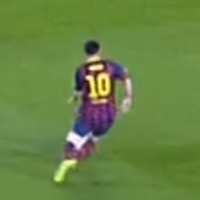
\includegraphics[width=.4\linewidth]{./images/resize_barcelona2.png}
        \captionof{figure}{En la imagen se observa la falta de resolución. Los
        bordes se ven difusos.
        \label{fig:barsa3}}
    \end{minipage}%
    \begin{minipage}[t]{.5\textwidth}
        \centering
        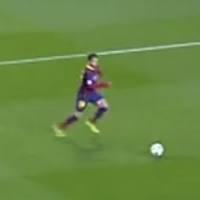
\includegraphics[width=.4\linewidth]{./images/resize_barcelona3.png}
        \captionof{figure}{Se observan dos de las dificultades del
        problema: la baja resolución y el diminuto tamaño de la pelota con
        respecto al jugador. \label{fig:barsa4}}
    \end{minipage}
\end{figure}

\subsection{Complejidad del Análisis en Tiempo Real}

Al tener una resolución de \textit{1080p} (aproximadamente dos millones de
píxeles por cuadro), el procesamiento de cada píxel debe tomar a lo sumo 20
nanosegundos. Para lidiar con esta restricción se puede utilizar información
adicional de la que se disponga respecto al video con el objeto de evitar
procesar píxeles de poca o nula utilidad para el seguimiento. Un ejemplo de
esto es descartar píxeles que estén fuera de la cancha, ya que es probable que
la cámara encuadre más que el campo de juego, abarcando las gradas, el público
espectador, publicidades alrededor del campo de juego, entre otros.

Muchos autores han desarrollado algoritmos automáticos de seguimiento de
objetos en secuencias de imágenes (ver \cite{IFTrace, alp, local-learning,
MHT-2}). Todos ellos están basados en soluciones de ecuaciones diferenciales en
derivadas parciales y proveen resultados precisos, pero tienen severas
restricciones que impiden que se utilicen para aplicaciones en tiempo real.

Para este trabajo, se utiliza el algoritmo de contornos activos (ver
\cite{fast-level-set}), el cual no utiliza ecuaciones diferenciales (haciéndolo
apto para aplicaciones en tiempo real) y además hace un análisis local de los
objetos seguidos en la imagen, lo cual hace que el tiempo de análisis de un
cuadro sea dependiente de la cantidad de píxeles que abarque la silueta de un
jugador e independiente de la resolución del video.

\subsection{Distorsión de la lente}

Al utilizar una única cámara para captar la cancha entera se corre el riesgo de
que los puntos de la imagen más alejados al foco de la cámara sufren una
distorción. Este es el llamado ``efecto de ojo de buey'' e introduce mucho
error, por ejemplo en la aplicación de la homografía, por lo tanto se debe
aplicar una corrección. Una lente apropiada y bien calibrada puede reducir este
error, pero nunca puede ser eliminado totalmente.

% TODO: Screenshots

\subsection{Oclusiones entre jugadores}

En un partido es muy común que ocurran oclusiones entre los jugadores. El
sistema debe poder tolerar la oclusión parcial o total de los jugadores. Esto
puede llevar a situaciones muy difíciles de detectar automáticamente. Por
ejemplo, una situación particularmente difícil de resolver se dá cuando dos
jugadores del mismo equipo (con vestimenta muy similar) se encuentren alineados
con respecto a la cámara. Una posible solución es utilizar información de
cuadros anteriores para estimar la velocidad de cada uno y estimar sus nuevas
posiciones, pero esto es poco efectivo si los jugadores cambian de velocidad
mientras uno ocluye al otro, o si la velocidad era muy similar al momento de
generarse la oclusión.

Una situación problemática similar es una jugada de tiro de esquina (córner),
donde las oclusiones entre varios jugadores son muy numerosas, lo que agrega a
la restricción de tiempo real mayor complejidad, ya que la resolución de
oclusiones debe ser muy eficiente en tiempo.



\newpage

\chapter{Descripción del Método}
\label{chap-ac}

En este Capítulo se describe el método de seguimiento seleccionado para este
trabajo. En primer lugar, la Sección \ref{sec:ac} explica el algoritmo
utilizado (\emph{Contornos Activos}), y en la Sección \ref{sec:impl} su
implementación. Luego, en la Sección \ref{sec:eleccion} se justifica la
elección del algoritmo. Finalmente, en la Sección \ref{sec:ac-problemas} se
analizan las limitaciones del algoritmo para esta aplicación.

\section{Contornos Activos}
\label{sec:ac}
La segmentación basada en contornos activos se basa en definir una región en
base a su contorno. El contorno o borde de una región $\Omega_i$ se representa
por una curva paramétrica dada por:

\begin{equation}
    C_i(s) = (x_i(s), y_i(s))
\end{equation}
donde $0 \leq s \leq S_i$, y $C_i(0) = C_i(S_i)$, siendo $S_i$ el total de
puntos que conforman la curva. Es decir, $C_i$ es una curva cerrada.

Se definen tantos contornos como objetos de interés haya en la secuencia ($i$
es un entero entre 1 y el número de objetos). Adicionalmente, se considera una
región $\Omega_0$ que contiene a todo punto que no forma parte de ninguna otra
región. Se la denomina \textit{región de fondo}.

Se declara una función de probabilidad $p$ que permite saber que tan probable
es que un píxel forme parte de una dada región. Para esto, es necesaria una
función $v$ que dado un píxel devuelve un vector $v(x)$ de características,
por ejemplo los valores RGB del píxel. Esto permite calcular $p(v(x) \vert
\Omega_i)$, la probabilidad de que un píxel $x$ forme parte de una región
$\Omega_i$. Estas funciones dependen de la secuencia particular a ser
analizada, por lo que varían dependiendo del caso de estudio. Como ejemplo, se
toman los valores RGB como vector de características y $p(v(x) \vert \Omega_i)
= \| v(x) - v_i \| $, donde $v_i$ es el valor promedio RGB de todo píxel en la
región $\Omega_i$.

Se define la función de energía de los contornos:

\begin{equation}
    \label{eq:ac-energy}
    E = - \sum_{m=0}^{M}{\int_{\Omega_m}{\log{p(v(x) \vert \Omega_m)} dx} + \lambda \int_{C_m}{ds}}
\end{equation}

Los algoritmos basados en contornos activos buscan minimizar esta ecuación. Si
el valor de $E$ es mínimo para un cuadro, se considera que se encontró la mejor
aproximación de la región de los objetos interés. De \ref{eq:ac-energy} se
deriva la ecuación de evolución de cualquier curva $C_m$:

\begin{eqnarray}
    \frac{dC_m}{dt} &=& (F_d + F_s) \overrightarrow{N}_{C_m} \\
    F_d &=& \log{p(v(x) \vert \Omega_m) / p(v(x) \vert \Omega_0)} \\
    F_s &=& \lambda \kappa_m \label{eq:ac-formal}
\end{eqnarray}

$F_d$ y $F_s$ son fuerzas derivadas de la ecuación de energía. $F_d$ representa
la competencia entre regiones y $F_s$ una función que produce el efecto de
suavizado. $\kappa_m$ es la curvatura de la curva $C_m$.

\section{Implementación Numérica}
\label{sec:impl}

Se toma de referencia la implementación según \citeauthor{fast-level-set} (ver
\cite{fast-level-set}). En la implementación, el borde de un contorno $C_m$ se
representa usando dos conjuntos de píxeles correspondientes a los bordes
interno y externo, $L_{in}$ y $L_{out}$ respectivamente. Entonces, la evolución
se realiza intercambiando píxeles entre estos dos conjuntos.

A continuación se detalla la técnica para la segmentación de un solo objeto de
interés que se puede fácilmente extrapolar y utilizar para la segmentación de
múltiples objetos
\footnote{Para la segmentación de múltiples objetos basta con marcar las
distintas regiones con un identificador distinto y seguirlas por separado.}.

El objeto de interés $\Omega_{1}$ y el fondo $\Omega_{0}$ cumplen
$\Omega_{1}\cup\Omega_{0} = I_{k}$, donde $I_{k}$ es la imagen del cuadro $k$
de la secuencia de imágenes, y $\Omega_{1}\cap\Omega_{0} = \emptyset$. Cada una
de las regiones está caracterizada por su vector característico $v_{m}, m =
\{0,1\}$.

Se define una función $\phi(x)$ que indica si un píxel $x$ pertenece a una
región o al fondo de la siguiente manera:

\begin{equation}
\phi(x) =
\left\{
    \begin{array}{ll}
        3  & \mbox{si } x \in \Omega_{0} \mbox{  y  } x \notin L_{out} \\
        1  & \mbox{si } x \in L_{out}\\
        -1  & \mbox{si } x \in L_{in}\\
        -3 & \mbox{si } x \in \Omega_{1} \mbox{  y  } x \notin L_{in} \\
    \end{array}
\right.
\end{equation}

Los conjuntos $L_{in}$ y $L_{out}$ se definen como

\begin{equation}
    L_{in} = \{ x \mbox{ es un píxel } \vert \mbox{    }  \phi(x) < 0 \mbox{ y } \exists y \in N_{4}(x) \mbox{ de modo que } \phi(y) > 0 \}
\end{equation}

\begin{equation}
    L_{out} = \{ x \mbox{ es un píxel } \vert \mbox{    } \phi(x) > 0 \mbox{ y } \exists y \in N_{4}(x) \mbox{ de modo que } \phi(y) < 0 \}
\end{equation}

donde $N_{4}(x) = \{ y \mbox{ es un píxel } \vert \mbox{   } |x-y| = 1 \}$, son
los píxeles vecinos del píxel $x$.

El algoritmo de segmentación se compone de dos etapas, ya que luego de la
especificación inicial de la curva en forma supervisada
\footnote{Podría no ser supervisada. Existen variantes con determinaciones
semi-supervisadas del objeto de interés, así como también detección automática
basada en ciertas características predefinidas.}
se intercambian los píxeles de $L_{in}$ y $L_{out}$ en dos ciclos. En el
primero, se aplica la fuerza $F_{d}(x)$, y en el segundo se aplica $F_{s}(x)$
para la regularización.

En el primer ciclo, se ejecutan los siguientes pasos $N_{a}$ veces, donde $ 0 <
N_{a} < max(filas, columnas)$.

\begin{enumerate}

    \item Para cada $x \in L_{out}$, si $F_{d}(x) > 0$ entonces borrar $x$ de $L_{out}$ y agregarlo a $L_{in}$. \\
    Luego, $\forall y \in N_{4}(x)$, con $\phi(y) = 3$, agregar $y$ to $L_{out}$ y hacer $\phi(y) = 1$.

    \item Después del paso 1 algunos de los píxeles $x$ en $L_{in}$ pasan a ser píxeles internos. \\
    Por lo tanto, se sacan de $L_{in}$ y se hace $\phi(x) = -3$.

    \item Para cada $x \in L_{in}$ , si $F_{d}(x) < 0$ entonces, borrar $x$ de $L_{in}$ y agregarlo a $L_{out}$. \\
    Luego, $\forall y \in N_{4}(x)$, con $\phi(y) = -3$, agregar $y$ a $L_{in}$ y hacer $\phi(y) = -1$.


    \item Después del paso 3 algunos de los píxeles $x$ en $L_{out}$ pasan a ser píxeles externos. \\
    Por lo tanto, se sacan de $L_{out}$ y se hace $\phi(x) = 3$.

\end{enumerate}

En el segundo ciclo, la curva se suaviza utilizando un filtro Gaussiano, de tal
forma que la fuerza de evolución es $F_{s}(x) = G \otimes \phi(x)$. Para
aplicar $F_s$ se usan los mismos pasos que para $F_d$. El resultado final es
análogo a modificar la curva de acuerdo a la definición formal dada
anteriormente (Ecuación \ref{eq:ac-formal}).

En cada cuadro, el borde del contorno del objeto es actualizado de acuerdo al
resultado obtenido por el algoritmo en el cuadro anterior. En el caso de la
primera imagen, se puede dar de forma supervisada o semi-supervisada por el
usuario, o bien puede ser obtenida de forma automática mediante algoritmos de
aprendizaje complejos basados en características predefinidas.

El algoritmo termina cuando se alcanza la condición de corte, dada por las
ecuaciones \ref{eq:active-contours-stoppingCondition} o cuando se alcanza el
numero de iteraciones $N_a$

\begin{equation}
\label{eq:active-contours-stoppingCondition}
    \begin{array}{ll}
        F_{d}(x) \leq 0 & \forall x \in L_{out}\\
        F_{d}(x) \leq 0 & \forall x \in L_{in}
    \end{array}
\end{equation}

\section{Elección}
\label{sec:eleccion}

Se escogió el algoritmo \emph{Contornos Activos} por varios motivos:
\begin{itemize}
    \item No depende de disponer de bloques de $n \times n$ píxeles para su
        correcto funcionamiento. Una de las principales restricciones de este
        trabajo es utilizar una sola cámara para obtener el video, y, como se
        explica en la Sección \ref{sub-sec:camaras}, un jugador está formado
        por un número muy limitado de píxeles, dificultando el uso de
        algoritmos que no tengan esta característica.

    \item Su tiempo de ejecución no depende del tamaño del cuadro, sino del
        de los jugadores. Esto hace que el tiempo de procesamiento de un cuadro
        sea muy pequeño, posibilitando el análisis en tiempo real.

    \item Se cuenta con métodos de manejo de oclusiones para
        \emph{Contornos Activos}\cite{paper-juliana}.

\end{itemize}

\subsection{Parámetros}

Se seleccionaron experimentalmente los siguientes valores para las constantes
del método:

\begin{itemize}
\item $N_a = 500$ 
\item Para el filtro $G$, se usa una mascara de $7 \times 7$ con un $\sigma = 0.7$ 
\end{itemize}

\section{Limitaciones}
\label{sec:ac-problemas}

El correcto funcionamiento del algoritmo de contornos activos depende de una
buena selección de la función característica, para poder distinguir claramente
a un jugador respecto a otros objetos o respecto del fondo (ver
\cite{fast-level-set}). En casos como el ilustrado por la Figura
\ref{fig:camiseta}, elegir una función característica resulta sencillo, ya que
con elegir el color de la camiseta se asegura una buena descripción del
contorno a seguir. Sin embargo, la imagen de la Figura
\ref{fig:camiseta-rayada} introduce uno de los problemas en la selección de
esta función. Se puede ver que las diferencias entre ambos colores del objeto
hacen difícil identificarlos a ambos con una misma característica. Si se toma
el promedio del valor \textit{RGB}, considerando que el color negro tiene valor
$(0, 0, 0)$ y el rojo $(255, 0, 0)$, el promedio de ambos seria $(127, 0, 0)$
(un marrón oscuro). Este valor muestra distinto a ambos colores, y no describe
bien a ninguno. Es por eso, que en la Figura \ref{fig:camiseta-rayada} el 
algoritmo de contornos activos podría determinar que uno de los dos colores de
la camiseta es más similar al fondo que al promedio, y en consecuencia
actualizar el contorno siguiendo únicamente uno de los dos colores.

\begin{figure}[H]
    \centering
    \begin{minipage}[t]{.5\textwidth}
        \centering
        
\includegraphics[width=.4\linewidth]{./images/rect2995.png}
        \captionof{figure}{Camiseta de color lisa. El color de la camiseta es
          claramente distinguible del fondo.
          \label{fig:camiseta}
        }
    \end{minipage}%
    \begin{minipage}[t]{.5\textwidth}
        \centering
        
\includegraphics[width=.4\linewidth]{./images/rect2996.png}
        \captionof{figure}{Camiseta de 2 colores a rayas. Uno de los dos
          colores es más similar al color de fondo que al promedio.
          \label{fig:camiseta-rayada}
        }
    \end{minipage}
\end{figure}

Este es un desafío grande debido principalmente a dos problemas:
\begin{itemize}

\item Selección de colores: si la cancha tiene un color muy similar a la
  camiseta de un equipo, ¿cómo será posible distinguirlos? En este trabajo se
  exploran distintas alternativas, como utilizar distintas codificaciones de
  color.

\item Textura de los jugadores: esto representa un gran problema por varias
  razones. La primera es que la técnica de contornos activos depende de la
  selección de una o varias características del objeto a seguir. Como la
  característica más distintiva es el color, la técnica se basa en ella. Pero
  para camisetas con más de un color, encontrar un único color característico
  no es posible. Esta dificultad se ilustra en la imágenes de las figuras
  \ref{fig:barsa1} y \ref{fig:barsa2}. Por otro lado, dada la escasa cantidad
  de píxeles que representan a un jugador, debido al enfoque de única
  cámara de este trabajo, cualquier tipo de análisis se torna complejo cuando
  sus características no están lo suficientemente definidas como para
  diferenciarlas (ya sea de otros jugadores o del fondo).

\end{itemize}

\begin{figure}[H]
    \centering
    \begin{minipage}{.5\textwidth}
        \centering
        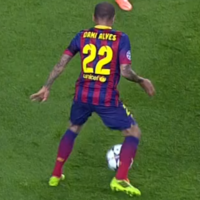
\includegraphics[width=.4\linewidth]{./images/resize_barcelona1.png}
        \captionof{figure}{Desde este punto de vista, se puede observar al
        menos 3 fuertes características (colores) en la camiseta del jugador,
        rojo, azul y amarillo.}
        \label{fig:barsa1}
    \end{minipage}%
    \begin{minipage}{.5\textwidth}
        \centering
        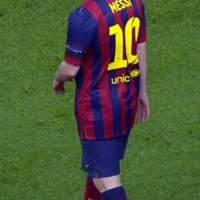
\includegraphics[width=.4\linewidth]{./images/resize_barcelona4.png}
        \captionof{figure}{Incluso con mayor resolución, las distintas
        características (como ser los colores azul, amarillo, y rojo)
        dificultan el seguimiento con contornos activos.}
        \label{fig:barsa2}
    \end{minipage}
\end{figure}

%TODO aca mepa que pueden ir varias imagenes.
% 1 de un tracking de de un jugador de remera blanca (podría ser PRE y POST, osea sin pintar y pintado)
% 1 de un tracking de un jugador de boca (again PRE y POST)
% 1 de la pelota? Para mostrar la cantidad infima de píxeles?

% eordano says: Me parece que este TODO quedó viejo, lo borro?


\newpage

\chapter{Solución propuesta}
\label{chap-solution}

En esta Sección se describen las técnicas aplicadas para lograr el seguimiento
de los jugadores. En primer lugar, se detallan algoritmos utilizados para
ignorar los elementos del fondo de la imagen en la Sección
\ref{sec:background-elimination}. Luego, se detalla cómo fue utilizado el
algoritmo contornos activos (ver \cite{fast-level-set}) y las modificaciones
que se le hicieron en la Sección \ref{sec:ac-extension}.

\section{Eliminación de fondo}

\label{sec:background-elimination}
Se evaluó que el análisis por contornos activos se beneficiaría de un análisis
previo que detecte e informe a la actualización del contorno sobre sectores de
los cuadros del video que sin duda no corresponden a las siluetas de los
objetos de interés para el seguimiento.

Con ese fin, se analizaron distintos métodos para extraer información adicional
de la imágen y detectar con el objetivo de ignorar sectores de la imágen que no
correspondan a jugadores con total certeza. A continuación se describen los
métodos evaluados.

\subsection{Tribuna y publicidades}
\label{subsec:crop-tribunas}

La técnica más simple de eliminación de sectores es una técnica de
\textit{recorte} que elimina de la imágen todo píxel ajeno a un polígono
(como puede ser un cuadrilátero) que bordea la cancha. En las Figuras
\ref{fig:crop-antes} y \ref{fig:crop-despues} se muestra el resultado
de aplicar esta técnica a uno de los videos utilizados en el trabajo.

\begin{figure}[H]
  \centering
    \begin{minipage}[t]{.45\textwidth}
      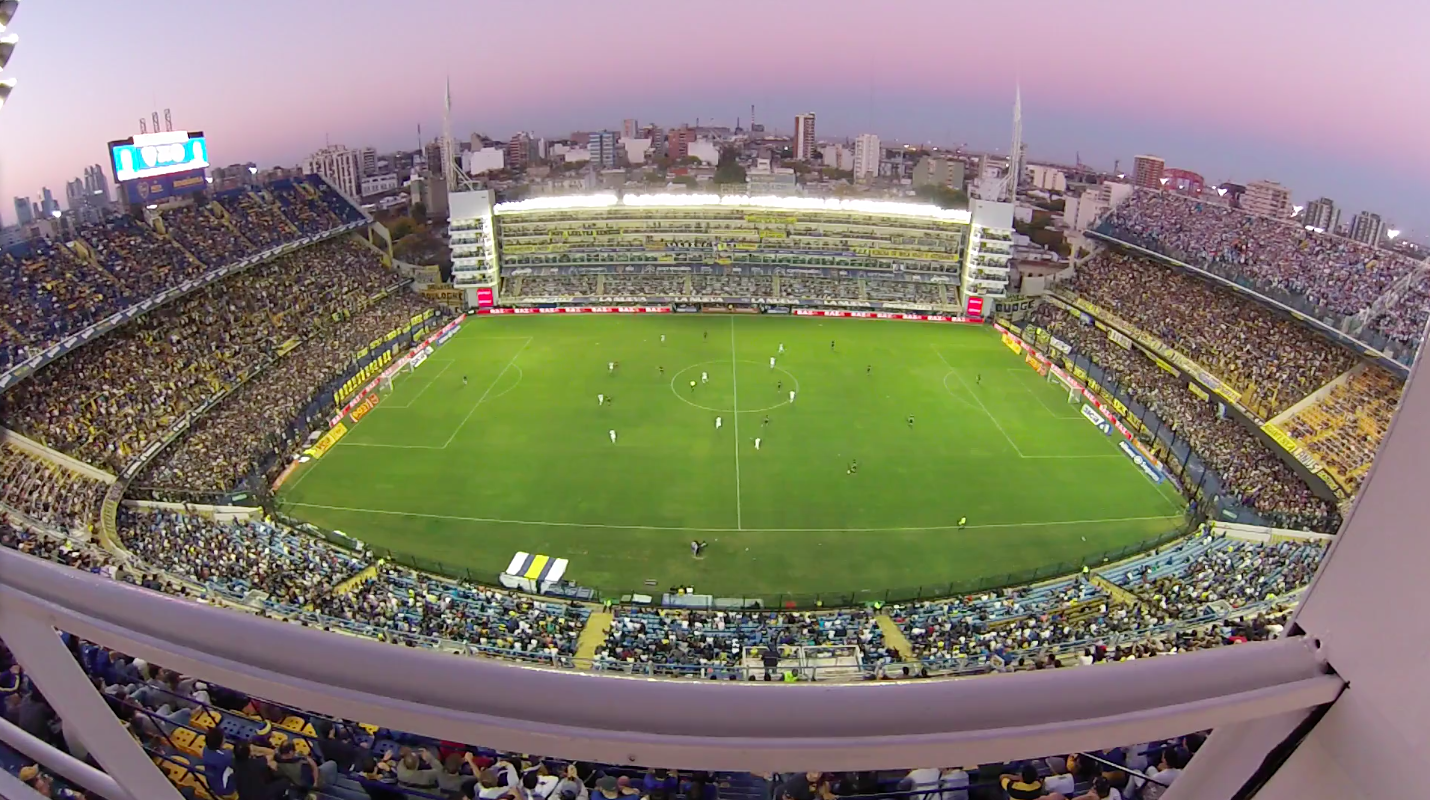
\includegraphics[width=\linewidth]{./images/Crop_Antes.png}
      \caption{Un cuadro del video de un partido entre Boca e Independiente.
      \label{fig:crop-antes}}
    \end{minipage}
    \begin{minipage}[t]{.45\textwidth}
      \centering
      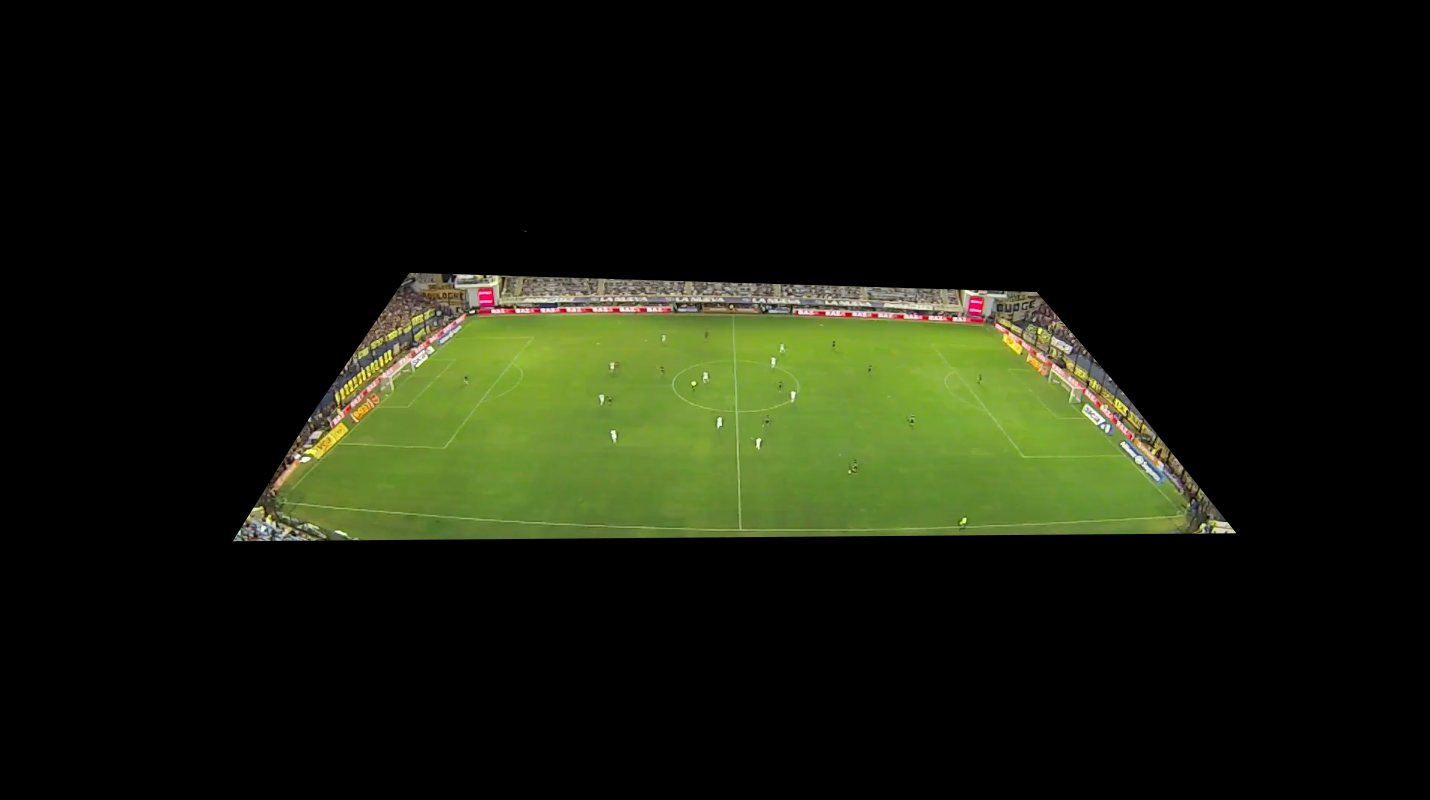
\includegraphics[width=\linewidth]{./images/Crop_Despues.png}
      \caption{El mismo cuadro, luego de aplicarle la operación \textit{recorte}.
      \label{fig:crop-despues}}
    \end{minipage}
\end{figure}

\subsection{Substracción de Fondo por Valor de Energía}

Se implementó el método de eliminación de fondo descripto en
\cite{papers-tanos}, para eliminación de sectores que corresponden al
verde del césped de la cancha o líneas pintadas sobre el mismo basado en una
medición de la variación del color de cada píxel (energía).

Este no resultó ser un método apropiado debido a que el sistema de codificación
del video generaba muchos falsos negativos, sobre todo \textit{glitches}
alrededor de las líneas de la cancha, lo que les otorgaba a estos puntos un
mayor valor de energía del que realmente tendrían. En la Figura \ref{fig:tanos-fondo-sin}
se muestra un recorte del primer cuadro del video de un partido entre Boca e Independiente.
En las figuras \ref{fig:tanos-fondo} y \ref{fig:tanos-fondo-broken} se muestra el
resultado de aplicar este algoritmo en ese mismo recorte. Se puede ver que en el cuadro
\#27 detecta muy bien el fondo, pero en el siguiente cuadro cambios en la imagen
hacen que descarte de manera erronea ciertas partes del fondo.

% TODO: el arquero se lo morfa
\begin{figure}[H]
  \centering
    \begin{minipage}[t]{.45\textwidth}
      
\includegraphics[width=\linewidth]{./images/tanos-fondo-f1.png}
      \caption{Recorte del cuadro \#1 del video de un partido entre Boca e Independiente
      \label{fig:tanos-fondo-sin}}
    \end{minipage}
    \begin{minipage}[t]{.45\textwidth}
      
\includegraphics[width=\linewidth]{./images/tanos-fondo-f27.png}
      \caption{Recorte del cuadro \#27 del video, con el fondo segun el algoritmo en azul.
      \label{fig:tanos-fondo}}
    \end{minipage}
    \begin{minipage}[t]{.45\textwidth}
      \centering
      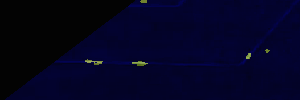
\includegraphics[width=\linewidth]{./images/tanos-fondo-f28.png}
      \caption{Recorte del cuadro \#28 del video, con el fondo segun el algoritmo en azul.
      \label{fig:tanos-fondo-broken}}
    \end{minipage}
\end{figure}

\subsection{Eliminación de Líneas}

Se encontro que las lineas blancas que delimitan la cancha y sus distintas partes
presentan un problema para el seguimiento de los equipos con camisetas blancas o de
colores claros. Para evitar que el algoritmo de contornos activos considere que las
lineas son parte de un jugador, como en la figura \ref{fig:confusion-linea}.

% TODO: Tebex, esto no parece coincidir co nel codigo...
% TODO: esta bien que digas que probamos, pero no decis cual es el posta
% TODO: Decis "analisis morfologico" es muuuuy poco explicativo
Basado en la detección de líneas de Hough, se desarrolló un método similar que
detecta los tramos pintados de blanco en el césped de la cancha. El mismo
funciona aplicando un detector de bordes (se probaron resultados utilizando
tanto el método de Roberts como el de Canny), umbralizando el resultado, y
haciendo un análisis morfológico de las componentes conexas obtenidas luego de
la umbralización.

\begin{figure}[H]
  \centering
    \begin{minipage}[t]{.45\textwidth}
      
\includegraphics[width=\linewidth]{./images/confusion-linea.png}
      \caption{Se muestra como el contorno incluye parte de la linea
      \label{fig:confusion-linea}}
    \end{minipage}
\end{figure}

\subsection{Eliminación del césped}
\label{sec:cesped}

Para la eliminación del césped del campo de juego se requiere caracterizarlo
de alguna forma. Para esto, se realiza un analisis de los colores de
la imagen recortada, es decir la imagen resultante luego aplicar la técnica
de \textit{recorte}, detallada en \ref{subsec:crop-tribunas}, una vez seleccionados
los contornos iniciales de los jugadores. Sobre este cuadro, se calcula el valor
promedio y desvio estandard de todo pixel que no forme parte de los jugadores o
un elemento ya conocido del fondo (por ejemplo, las lineas). 

Con este valor, se considera parte del césped cualquier punto que no tenga las
caracteristicas de un jugador (segun definidas en la sección \ref{sec:caracteristicas}),
y se encuentre a menos de 3 desvios del color promedio calculado.

\section{Contornos activos}
\label{sec:ac-extension}

Como se explica en Sección \ref{sec:ac-problemas}, cuando los objetos de
interés son complejos, la utilización del color promedio como única
característica distintiva no alcanza. Es por esto que varias de las mejoras
planteadas al algoritmo de contornos activos giran en torno a la selección de
características para representar a los objetos de interés. Esta Sección
describe cambios que se han incorporado para hacer el algoritmo más efectivo
ante un video correspondiente a un partido de fútbol.

Si bien el color promedio resulta insuficiente para caracterizar correctamente
al objeto, puede utilizarse en complemento con otras características. Una opción
es la utilización de la varianza de color en el objeto de interés.

Además de estos indicadores estadísticos, se pueden utilizar varias valores
para caracterizar el objeto, en lugar de utilizar un solo valor como puede ser
el color promedio o la varianza. Para esto, por ejemplo, puede realizarse un
histograma de colores y seleccionar los picos más altos del histograma como
colores representativos del objeto.

\subsection{Características}
\label{sec:caracteristicas}

Se estudiaron varias posibilidades para la selección de características que
determinaran los contornos de los jugadores respecto al color de fondo.
Finalmente, se optó por utilizar tres características, correspondientes a los
valores de RGB de cada píxel. A continuación se detallan alternativas:
\begin{itemize}
  \item \textbf{Valores HSL}: Se tomaron, en vez de los valores de rojo, verde
    y azul, los valores de \textit{hue}, \textit{saturation} y
    \textit{lightning}.

  \item \textbf{Desviación Estándar}: Se tomaron seis características para cada
    píxel: color (RGB o HSL) y desviación estándar de ese píxel respecto a los
    demás píxeles en una ventana de 3x3 píxeles alrededor del mismo.

\end{itemize}

\subsubsection{Selección de características}

Las características de un jugador son seleccionadas en base a los valores
encontrados inicialmente dentro de un cuadrado de un ancho y alto especificado
por el operador, que depende del video siendo analizado. Entre los píxeles
abarcados por el área de ese cuadrado, se calcula el promedio y desvio estandard
de todos ellos. La caracteristica del jugador queda entonces definida por el
vector $v = (r_a, g_a, b_a, r_{dev}, g_{dev}, b_{dev})$, donde los primeros
tres valores representan el promedio de los componentes \textit{RGB} y los ultimos
tres el desvio standard de los componentes \textit{RGB}.

El vector de caracteristicas del fondo tiene la misma forma, y se construye
utilizando los valores calculados en la Sección \ref{sec:cesped}.

\subsubsection{Aprendizaje de valores}

Se realiza un aprendizaje simple para las características de cada contorno. En
cada cuadro, siendo las características de un contorno dado un vector
$\mathbf{v}$, se calcula el promedio de los valores de las características para
todos los píxeles pertenecientes al contorno y se lo denomina
$\hat{\mathbf{v}}$. A continuación se actualiza $\mathbf{v}$ y se lo reemplaza
por un nuevo valor $\mathbf{v_n}$ calculado de acuerdo a:

\[
  \mathbf{v_n} = \left(1-\alpha\right)\mathbf{v} + \alpha \hat{\mathbf{v}}
\]

Se toma un valor de $\alpha$ del orden de $10^{-2}$, es decir, se toma el $1\%$
de $\hat{\mathbf{v}}$. Esto evita la posibilidad de que se memorize cambios
no deseados, como lo podria ser una oclusion parcial, antes de su correción.



\newpage

\chapter{Resultados}
\label{chap-results}

Este Capítulo presenta un análisis de los resultados obtenidos a partir de la
ejecución del algoritmo utilizando distintos videos. A lo largo de esta Sección
se refiere al \textit{algoritmo} como a la versión modificada de contornos
activos que fue descripta en el Capítulo \ref{chap-solution}. Las palabras
\textit{aplicación} y \textit{programa} serán utilizadas indistintamente para
referirse al programa que implementa dicho algoritmo, junto con una interfaz de
usuario para el operador. Se refiere a la \textit{implementación} como la parte
del programa que implementa el algoritmo.

En primer lugar, la Sección \ref{sec:aplicacion} describe la aplicación, los
datos que deben ser provistos por el operador, y el funcionamiento de la misma.
La Sección \ref{sec:evaluacion} presenta los resultados obtenidos de la
ejecución del programa y las métricas utilizadas para evaluar la performance de
la implementación. Por último, en la sección \ref{sec:iftrace} se presenta la
comparación con otro método de seguimiento.

\section{Aplicación}
\label{sec:aplicacion}

El programa incorpora una interfaz gráfica utilizada tanto para dar
instrucciones como para recibir información acerca del partido y del
funcionamiento del algoritmo. La misma cuenta con una sección donde se muestra
una lista de los jugadores que están siendo seguidos, una donde se puede
visualizar el video original con un recuadro en cada jugador seguido, un mapa de
calor que muestra las posiciones más frecuentes, y una imagen que permite al
operador evaluar cualitativamente el correcto funcionamiento del algoritmo. Se
puede ver una captura de pantalla de la aplicación en la Figura
\ref{fig:screen1}.

\begin{figure}
    \centering
    \captionsetup{justification=centering}
    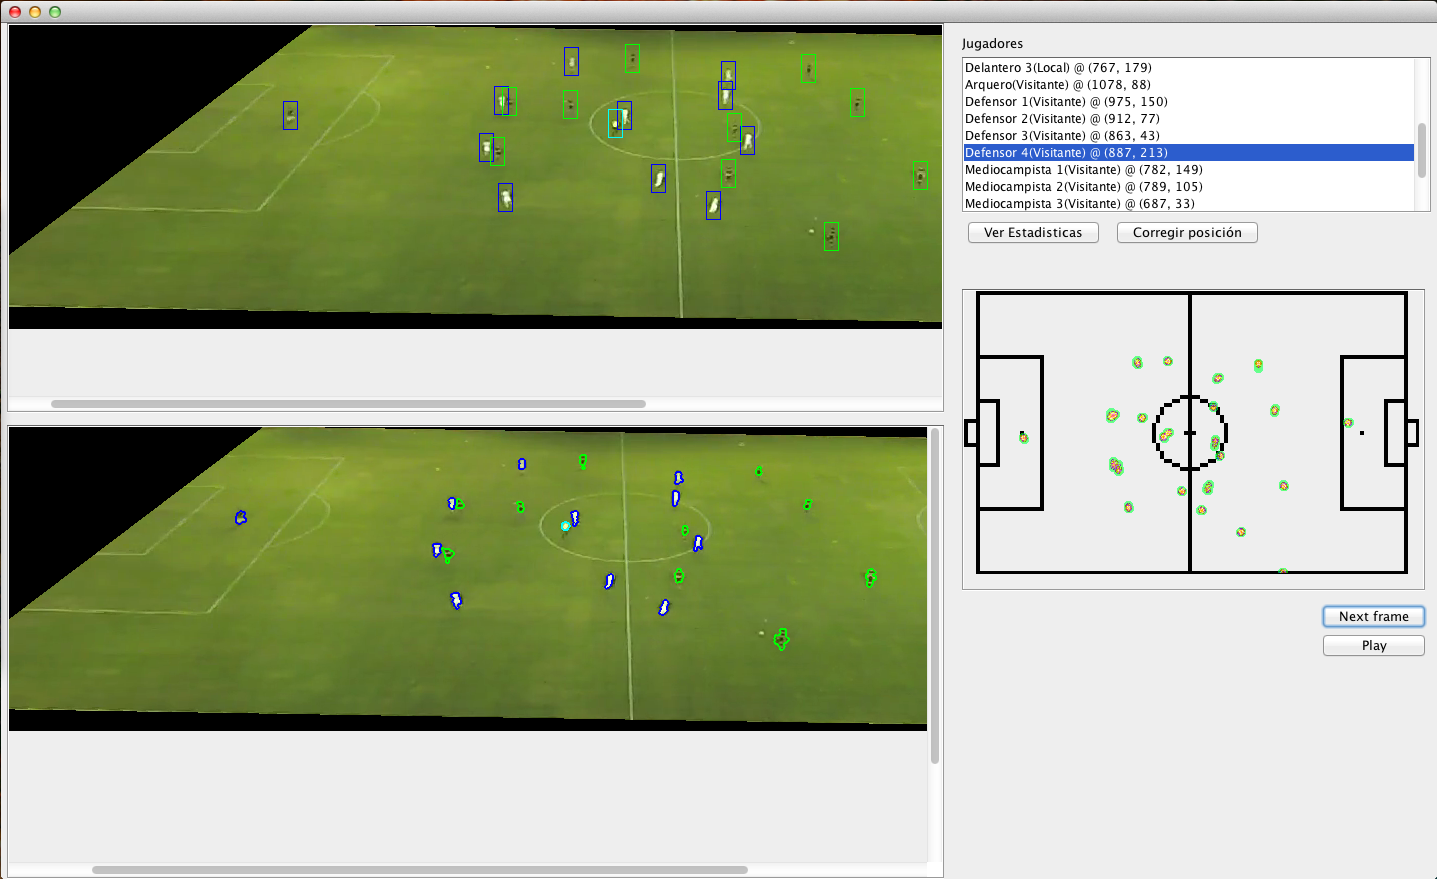
\includegraphics[width=\linewidth]{./images/Screen-Boca.png}
    \captionsetup{justification=centering}
    \caption{Captura de pantalla de la aplicación, mostrando el seguimiento en un video de fútbol.}
    \label{fig:screen1}
\end{figure}

Para comenzar la ejecución del algoritmo, el programa requiere que el operador
identifique la posición de los jugadores en la imagen inicial de la secuencia.
En este paso, también debe agregar información acerca del número de camiseta
que viste, el equipo al cual pertenece y el nombre de cada jugador. Se puede
obtener información de un jugador específico mediante la lista de jugadores
seguidos en la esquina superior derecha. La Figura \ref{fig:screen-jugador}
muestra el detalle con información de un jugador luego de unos segundos de
seguimiento.

\begin{figure}[H]
    \centering
    \captionsetup{justification=centering}
    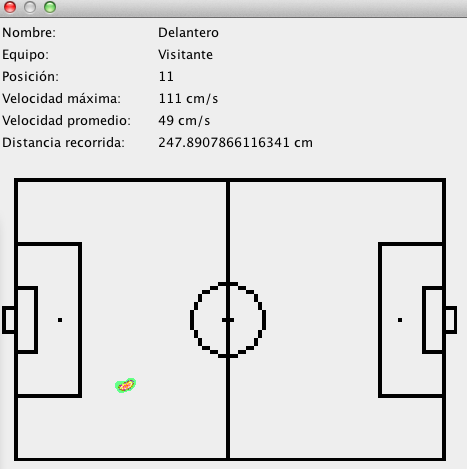
\includegraphics[width=0.60\linewidth]{./images/Screen-Jugador-Stats.png}
    \caption{Captura de pantalla de la aplicación, que muestra información del seguimiento de un jugador.}
    \label{fig:screen-jugador}
\end{figure}

Un paso adicional que debe ejecutar el operador es determinar los puntos a
utilizar para el cálculo de la homografía. Los datos necesarios para ello son
cuatro parejas de puntos, como se explica en la Sección \ref{sec:homography}. De
estas parejas, el primer punto es una coordenada de la imagen en perspectiva y
el otro punto es la coordenada en un plano bidimensional. Con cuatro de estas
relaciones, se puede calcular la matriz que resuelve la homografía para
cualquier otro punto.

Una vez que el programa tiene estos datos, el algoritmo puede comenzar su
ejecución. Existen dos modos: en un modo se puede avanzar un cuadro sólo ante la
indicación del operador (en una mecánica de tipo ``cuadro por cuadro'') y en
otro modo se puede avanzar automáticamente cada vez que se computa un cuadro
(mecánica de tipo ``tiempo real'').

Para cada cuadro, se informa:
\begin{itemize}
\item Posiciones actualizadas de los jugadores
\item Velocidad actual, promedio y máxima de un jugador
\item Mapa de calor del recorrido de cada jugador
\item Mapa de calor del recorrido de todos los jugadores
\end{itemize}

Finalmente, en un archivo se guarda la posición de cada jugador para cada momento.
Y de manera opcional, en cada cuadro se guarda en disco duro una copia del estado
actual del seguimiento para referencia futura.

\section{Material utilizado}

Se utilizaron principalmente dos videos, uno correspondiente a un partido entre
los equipos argentinos de los clubes Boca Juniors e Independiente; y un segundo
video en el cual se enfrentan los equipos Independiente y San Lorenzo. Se
detalla a continuación las características de las imágenes extraídas de esos
videos.

\begin{itemize}

  \item \textbf{Boca vs. Independiente:} El video cuenta con una resolución de
    \textit{1080p} (1920 píxeles de ancho y 1080 de alto). La cancha se muestra
    en su totalidad, y se puede observar las gradas del lado
    opuesto y cielo por encima de ellas. Luego de descartar esas regiones del
    video, la resolución pasa a ser de 1459 píxeles de ancho por 304 de alto.
    Se puede apreciar en la Figura \ref{fig:boca-figura} un cuadro del video, luego
    de la extracción de las gradas y corrección del efecto de curvatura de la
    lente.

    Los jugadores de Independiente usan remera y shorts de color blanco,
    fácilmente identificables respecto al fondo de color verdoso. El árbitro, de
    amarillo, también contrasta respecto al fondo. Los jugadores de Boca, por
    otro lado, son difíciles de identificar a la distancia y son confundidos con
    el color del césped de la cancha, como se ilustra en la Figura \ref{fig:boca-dificil-1}.

  \item \textbf{Independiente vs. San Lorenzo:} También filmado en resolución de
      \textit{1080p}, las esquinas del campo de juego quedan fuera del campo
      visual. El video fue editado con anterioridad y el alto de un cuadro es
      menor al alto de un video en resolución \textit{1080p}. Luego de descartar
      las gradas, la resolución final del video es de 1920 píxeles de ancho y
      540 de alto. La Figura \ref{fig:independ-figura} muestra un cuadro del
      video procesado.

    Los jugadores de ambos equipos, al utilizar los valores RGB de cada píxel,
    contrastan contra el césped y el algoritmo de contornos activos funciona
    correctamente al analizarlo cualitativamente.

\end{itemize}

\begin{figure}[H]
  \centering
  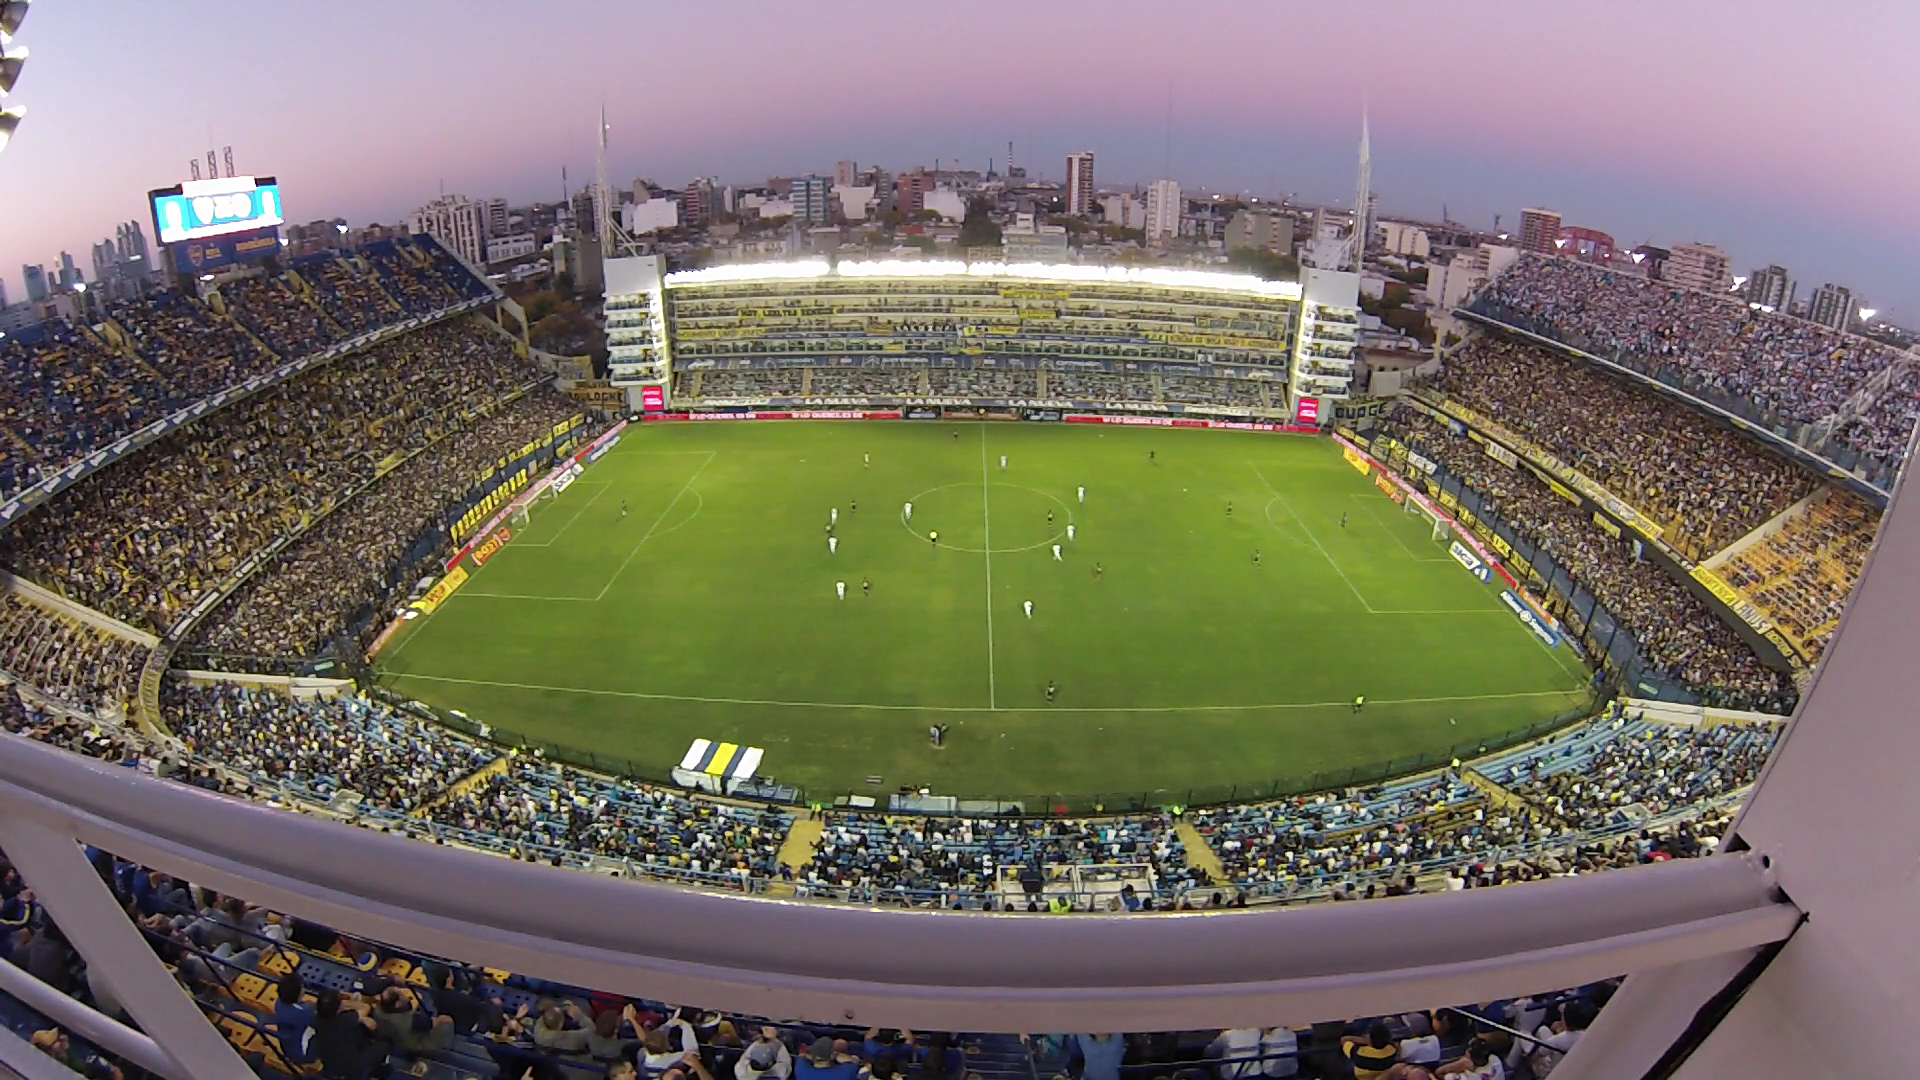
\includegraphics[width=\linewidth]{./images/boca-figura.png}
  \caption{Cuadro del video del partido entre Boca e Independiente.}
  \label{fig:boca-figura}
\end{figure}
\begin{figure}[H]
    \centering
    \captionsetup{justification=centering}
    \begin{minipage}[t]{.5\textwidth}
        \centering
        
\includegraphics[width=.4\linewidth]{./images/boca-dificil1.png}
    \end{minipage}%
    \begin{minipage}[t]{.5\textwidth}
        \centering
        
\includegraphics[width=.4\linewidth]{./images/boca-dificil2.png}
    \end{minipage}
    \caption{Acercamiento a dos jugadores en el video de Boca vs.
             Independiente. De acuerdo a la iluminación, se puede notar que el
             contorno de un jugador puede resultar muy difícil de delimitar.
        \label{fig:boca-dificil-1}}

\end{figure}
\begin{figure}[H]
  \centering
  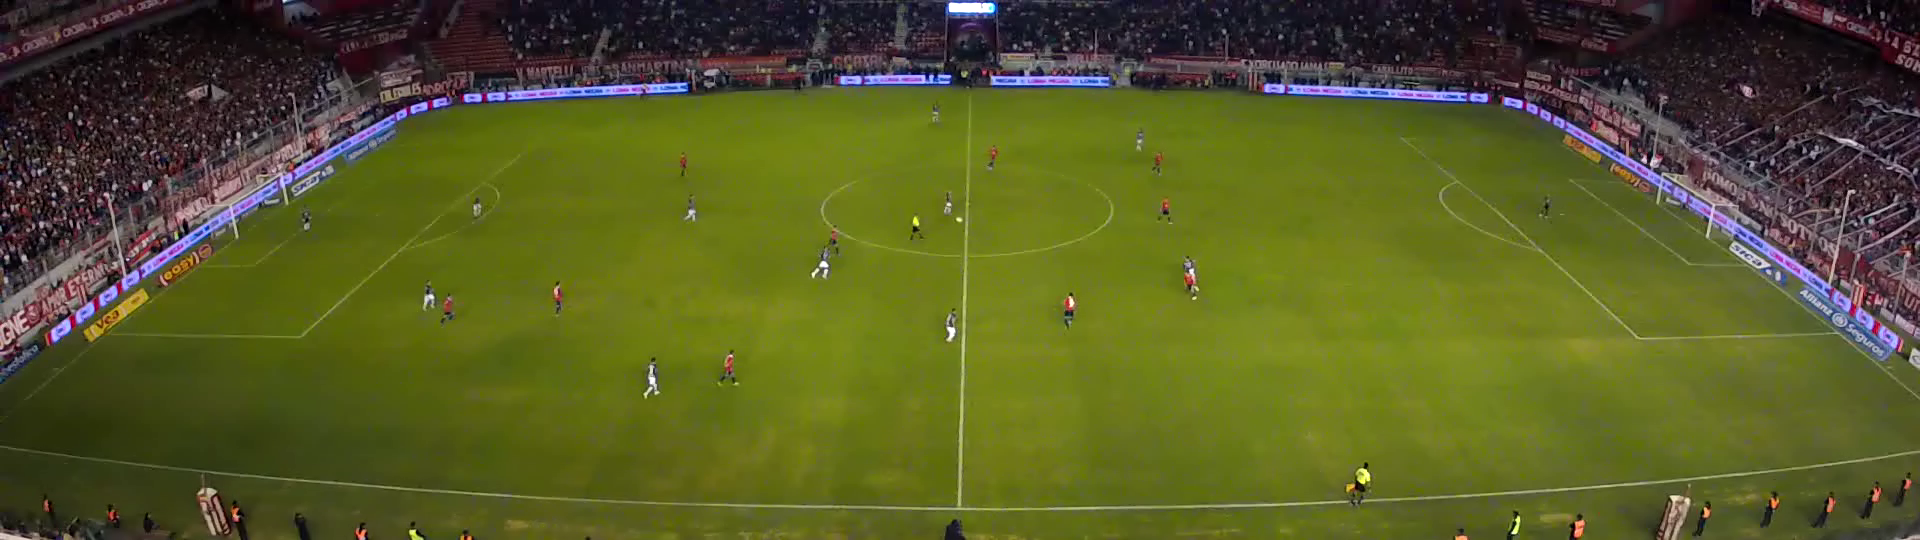
\includegraphics[width=\linewidth]{./images/independ-figura.png}
  \caption{Cuadro del partido en el que Independiente enfrenta a San Lorenzo.}
  \label{fig:independ-figura}
\end{figure}

Además, se tomaron pequeños cortes de tres videos de fútbol televisado, en los
cuales la cámara se encuentra prácticamente estática y se analizó la
correctitud del seguimiento en estos casos, contando con mayor resolución pero
sin poder efectuar exitosamente la eliminación de fondo o la aplicación de una
homografía para determinar las posiciones correctamente, ya que cada cuadro
donde la cámara cambia su orientación, la matriz de la homografía debería ser
recalculada con nuevos datos.

Los videos televisados utilizados pertenecen a tres partidos disputados durante
el año 2014. De la liga \textbf{UEFA}, se tomaron recortes de los partidos
\textbf{Manchester City vs Barcelona FC}, \textbf{Real Madrid vs Borussia
Dortmound}, y de la \textbf{FIFA World Cup} se tomaron fragmentos del partido
de cuartos de final de \textbf{Argentina vs Suiza}.

Del primer video televisado se extrajeron tres escenas en particular. En la
Figura \ref{fig:manchester1} se muestran algunos cuadros de estos fragmentos.
El video cuenta con una resolución de \textit{720p} (1280 píxeles de ancho por
720 píxeles de alto). Los jugadores de Manchester City, con su vestimenta
deportiva de color blanco, son confundidos por sus características con el color
de las líneas de la cancha. En el primer recorte, los jugadores son
correctamente identificados durante los 120 cuadros, exceptuando aquellos que
atraviezan una línea de cancha. Se corrigen correctamente dos oclusiones
parciales entre jugadores. En el segundo fragmento, los jugadores son
correctamente localizados a pesar de la alta velocidad de \textit{panning} de
la cámara. En el tercer video todos los jugadores, al igual que en el primero,
son correctamente localizados durante todo el video exceptuando aquellos que se
intersectan con las líneas marcadas en el césped.

En los otros dos videos se observaron similares características al video de
Manchester City, el seguimiento funciona correctamente bajo la asunción de que
los jugadores no estén ocluyendo una línea en el césped. La Figura
\ref{fig:realmadrid} muestra un cuadro donde se puede apreciar los colores de
la camiseta de ambos equipos en el partido \textbf{Real Madrid vs Borussia
Dortmound} y en la Figura \ref{fig:argentina1} se observa una captura del
partido de \textbf{Argentina vs Suiza}.


\begin{figure}[H]
    \centering
    \captionsetup{justification=centering}
    \begin{minipage}[t]{.45\textwidth}
        \centering
        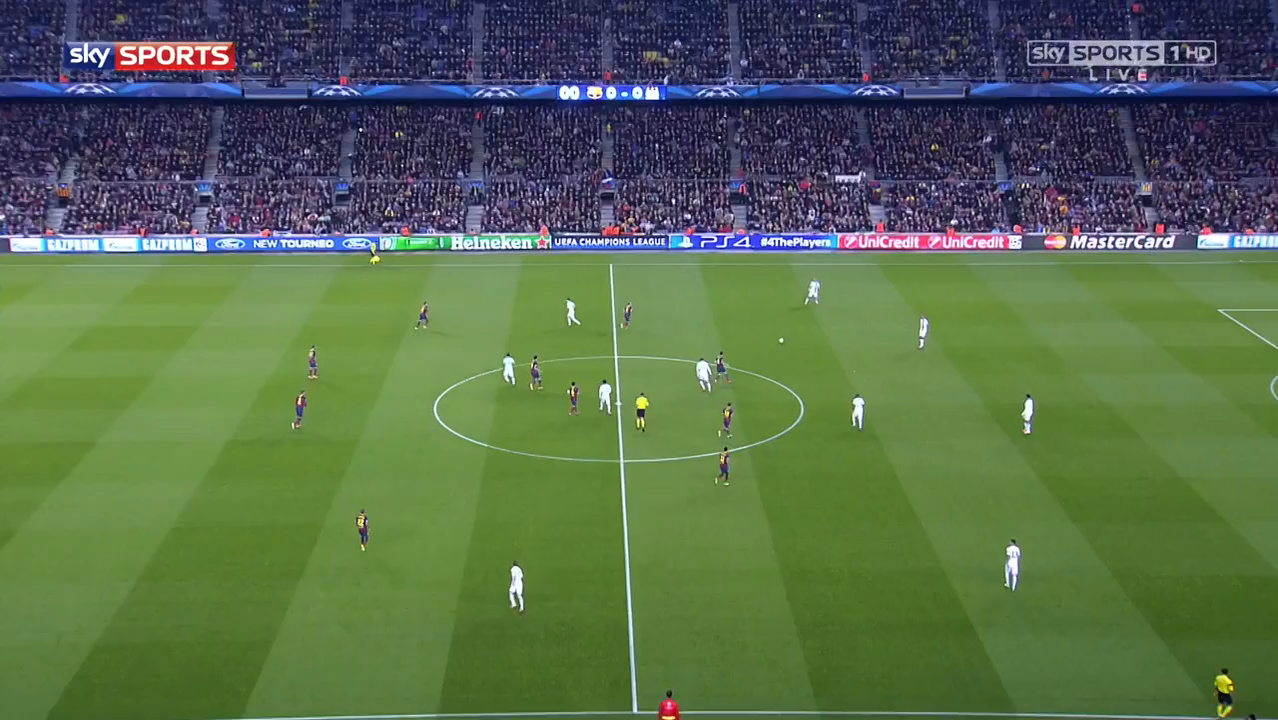
\includegraphics[width=\linewidth]{./images/manchester1.png}
    \end{minipage}%
    \vspace{0.1cm}
    \begin{minipage}[t]{.45\textwidth}
        \centering
        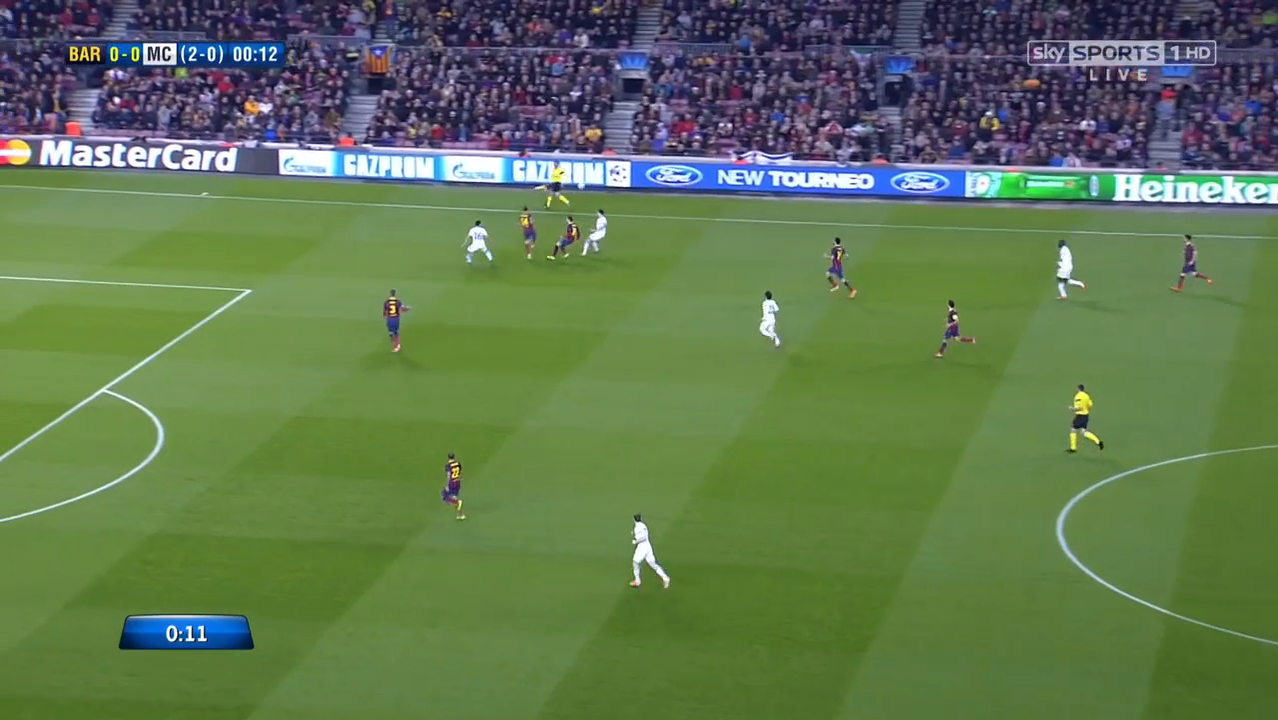
\includegraphics[width=\linewidth]{./images/manchester2.png}
    \end{minipage}
    \caption{Fragmentos del video televizado de un partido entre los equipos Manchester City y Barcelona FC.
        \label{fig:manchester1}}
\end{figure}

\begin{figure}[H]
    \centering
    \captionsetup{justification=centering}
    \begin{minipage}[t]{.45\textwidth}
        \centering
        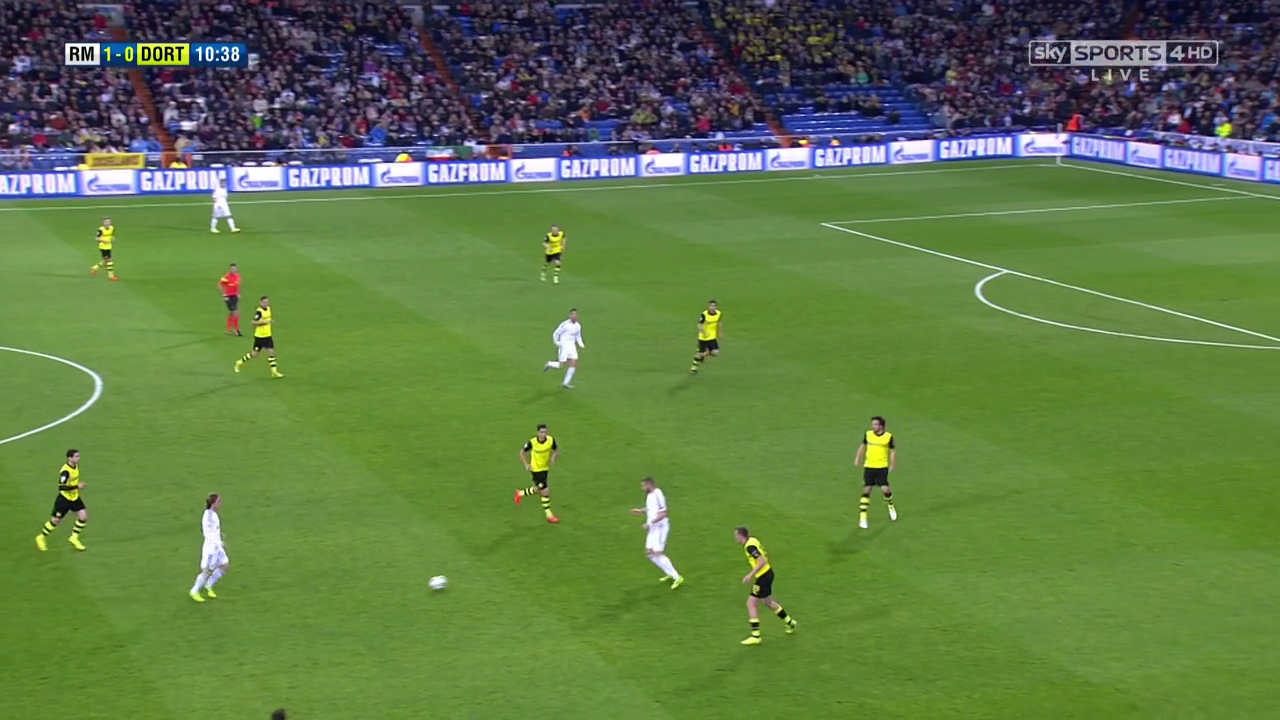
\includegraphics[width=\linewidth]{./images/realmadrid1.png}
        \caption{Real Madrid vs Borussia Dortmound, UEFA Champions League
        \label{fig:realmadrid}}
    \end{minipage}%
    \vspace{0.1cm}
    \begin{minipage}[t]{.45\textwidth}
        \centering
        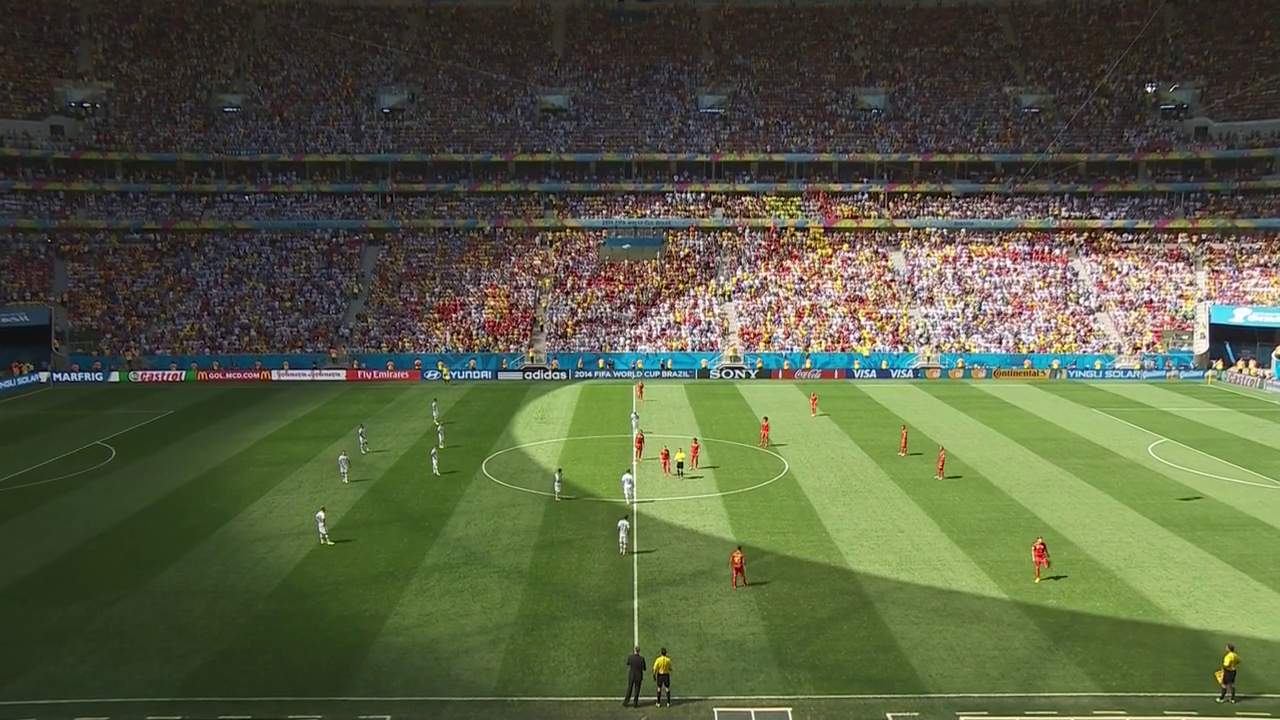
\includegraphics[width=\linewidth]{./images/argentina1.png}
        \caption{Argentina vs Suiza, FIFA World Cup 2014
        \label{fig:argentina1}}
    \end{minipage}
\end{figure}

\section{Evaluación del método}
\label{sec:evaluacion}

La principal evaluación del correcto funcionamiento del algoritmo es llevada a
cabo por el operador de forma cualitativa, como ocurre en otros trabajos
citados en el estado del arte (ver \cite{papers-tanos}). El resultado que
arroja está evaluación es positivo, consiguiéndose seguir correctamente a
todos los jugadores en casi todo momento. Sin embargo, existen algunas
situaciones en las que el algoritmo falla en el seguimiento y no logra
recuperarse por sí mismo, requiriendo una correción manual por parte del
operador para continuar su funcionamiento. Esto se atribuye a la baja calidad
de los videos utilizados como material y a la poca capacidad de procesamiento
en comparación (el poder de procesamiento de una sola computadora limita
algunas operaciones o técnicas).

Las situaciones en que se producen estos errores están bien identificadas
y ocurren porque el algoritmo, en una situación de proximidad entre dos
jugadores, a veces confunde a la sombra del otro jugador con el jugador
al cual se encuentra siguiendo, y comienza a seguir a la sombra, perdiendo
al jugador.

Para evaluar estos inconvenientes se define una métrica que mide exactamente la
cantidad de errores por unidad de tiempo. Esta métrica, resumida como la
cantidad de errores del algoritmo por cada cien cuadros, se intenta minimizar
durante el estudio de las variantes de la aplicación.

La ejecución del algoritmo utilizando el video entre Boca e Independiente
resulta en 7 errores en 766 cuadros, dando aproxidamente 0.91 errores cada cien
cuadros, lo que significa un poco menos de un error cada 4 segundos.

En el video del partido entre Independiente y San Lorenzo el algoritmo incurre
en 6 errores en 213 cuadros, dando 2.81 errores cada cien cuadros. Es decir,
algo menos de 3 errores cada 4 segundos.

Otro aspecto importante a la hora de evaluar la solución propuesta es su
velocidad, medida en el tiempo de ejecución que requiere para llevar a cabo su
trabajo. Para medir esto se define la métrica del tiempo que le toma al
algoritmo procesar un solo cuadro, o, lo que es lo mismo, la cantidad de
cuadros procesados por segundo. El objetivo es minimizar esta métrica
intentando acercarse lo más posible a los $24$ cuadros por segundo (equivalente
a $42$ milisegundos por cuadro), la velocidad de los videos utilizados.

\section{Comparación con IFTrace}
\label{sec:iftrace}

El algoritmo de seguimiento IFTrace, propuesto por \citeauthor*{IFTrace}, es un
algoritmo robusto que soporta cambios de iluminación y forma, oclusiones y se
centra en hallar características representativas de la textura de los objetos a
seguir. Es capaz de recuperarse de errores menores y permite el seguimiento de
múltiples objetos a la vez.

Un algoritmo de este tipo podría proporcionar una solución al problema. Para
comprobarlo, se llevaron a cabo algunas pruebas utilizando un video sintético
creado para este fin, y un video real de un partido de fútbol. En la Figura
\ref{fig:screen1} de la sección anterior se observa un video real. La figura
\ref{fig:sample-happy-occluded} muestra el primer cuadro del video sintético. Pueden
apreciarse a simple vista las marcadas diferencias entre ambos videos, como por
ejemplo la resolución de la imagen y el tamaño y la complejidad de los objetos
de interés.

\begin{figure}[H]
    \centering
    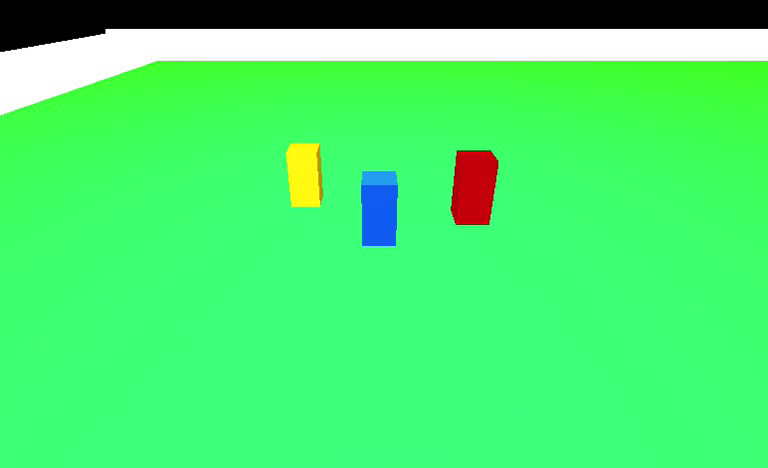
\includegraphics[width=\linewidth]{./images/sample_happy_occluded.png}
    \caption{Muestra de un cuadro del video sintético de prueba.}
    \label{fig:sample-happy-occluded}
\end{figure}

Como se puede ver en la Figura \ref{fig:happy-occluded-iftrace}, IFTrace logra
un correcto seguimiento de múltiples objetos en el video sintético. También
puede observarse, en la Figura \ref{fig:boca-iftrace}, como sigue correctamente
a un jugador en el video real. Sin embargo, el seguimiento sólo es exitoso
durante unos pocos cuadros, ya que, en el cuadro 17, el algoritmo cae en un
error del cual sólo una corrección manual puede sacarlo. Este tipo de corrección
semi-supervisada no está contemplada en el algoritmo de IFTrace.

\begin{figure}[H]
    \centering
    \begin{minipage}[t]{.25\textwidth}
      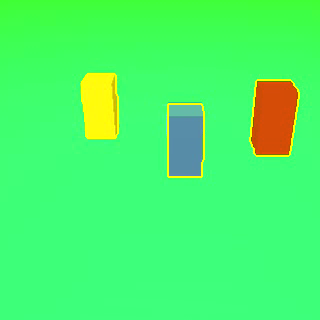
\includegraphics[width=1.4in]{./images/cropped_happy_occluded_00001.png}
      \centering
      \footnotesize
      \textbf{(a)} Cuadro 1
    \end{minipage}
    \hspace{-0.3cm}
    \begin{minipage}[t]{.25\textwidth}
      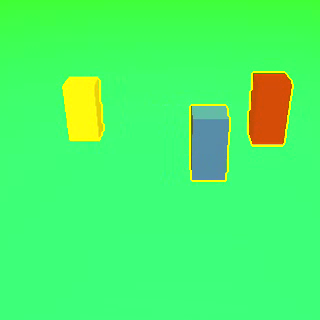
\includegraphics[width=1.4in]{./images/cropped_happy_occluded_00005.png}
      \centering
      \footnotesize
      \textbf{(b)} Cuadro 5
    \end{minipage}
    \hspace{-0.3cm}
    \begin{minipage}[t]{.25\textwidth}
      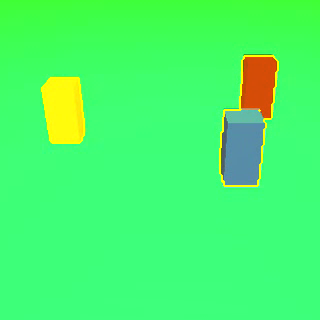
\includegraphics[width=1.4in]{./images/cropped_happy_occluded_00008.png}
      \centering
      \footnotesize
      \textbf{(c)} Cuadro 8
    \end{minipage}
    \hspace{-0.3cm}
    \begin{minipage}[t]{.25\textwidth}
      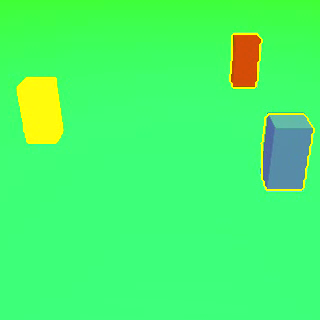
\includegraphics[width=1.4in]{./images/cropped_happy_occluded_00012.png}
      \centering
      \footnotesize
      \textbf{(d)} Cuadro 12
    \end{minipage}
    %% NASTY hack to make refernce work with figures and subfigures, put \label inside \caption env, little bird told me
    \caption{IFTrace funcionando en una secuencia de cuadros de video sintético.
    \label{fig:happy-occluded-iftrace}
    }
\end{figure}

\begin{figure}[H]
    \centering
    \begin{minipage}[t]{.25\textwidth}
      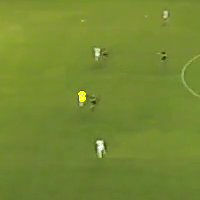
\includegraphics[width=1.4in]{./images/cropped_boca_00009.png}
      \centering
      \footnotesize
      \textbf{(a)} Cuadro 9
    \end{minipage}
    \hspace{-0.3cm}
    \begin{minipage}[t]{.25\textwidth}
      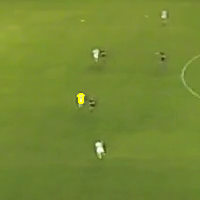
\includegraphics[width=1.4in]{./images/cropped_boca_00012.png}
      \centering
      \footnotesize
      \textbf{(b)} Cuadro 12
    \end{minipage}
    \hspace{-0.3cm}
    \begin{minipage}[t]{.25\textwidth}
      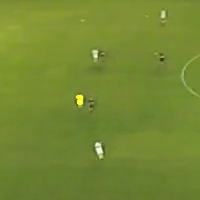
\includegraphics[width=1.4in]{./images/cropped_boca_00014.png}
      \centering
      \footnotesize
      \textbf{(c)} Cuadro 14
    \end{minipage}
    \hspace{-0.3cm}
    \begin{minipage}[t]{.25\textwidth}
      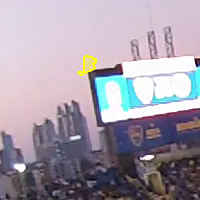
\includegraphics[width=1.4in]{./images/cropped_boca_00017.png}
      \centering
      \footnotesize
      \textbf{(d)} Cuadro 17
    \end{minipage}
    %% NASTY hack to make refernce work with figures and subfigures, put \label inside \caption env, little bird told me
    \caption{Seguimiento de un jugador en un video real utilizando IFTrace.
    \label{fig:boca-iftrace}
    }
\end{figure}

\begin{figure}[H]
    \centering
    \begin{minipage}[t]{.25\textwidth}
      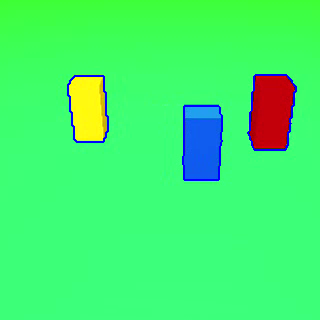
\includegraphics[width=1.4in]{./images/cropped_processing2.png}
      \centering
      \footnotesize
      \textbf{(a)} Cuadro 1
    \end{minipage}
    \hspace{-0.3cm}
    \begin{minipage}[t]{.25\textwidth}
      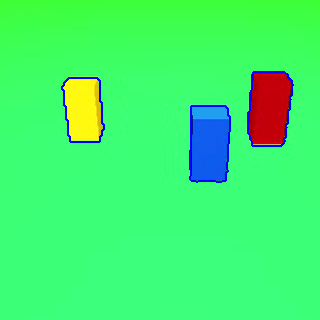
\includegraphics[width=1.4in]{./images/cropped_processing5.png}
      \centering
      \footnotesize
      \textbf{(b)} Cuadro 5
    \end{minipage}
    \hspace{-0.3cm}
    \begin{minipage}[t]{.25\textwidth}
      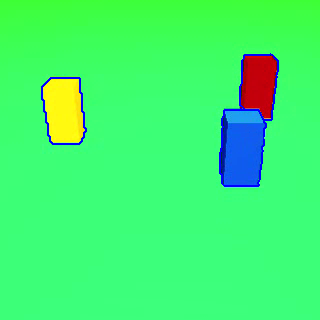
\includegraphics[width=1.4in]{./images/cropped_processing14.png}
      \centering
      \footnotesize
      \textbf{(c)} Cuadro 8
    \end{minipage}
    \hspace{-0.3cm}
    \begin{minipage}[t]{.25\textwidth}
      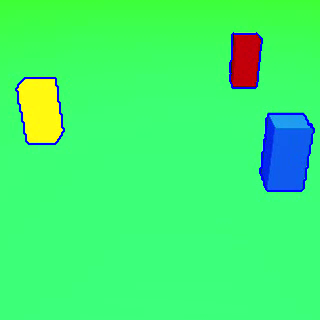
\includegraphics[width=1.4in]{./images/cropped_processing25.png}
      \centering
      \footnotesize
      \textbf{(d)} Cuadro 12
    \end{minipage}
    %% NASTY hack to make refernce work with figures and subfigures, put \label inside \caption env, little bird told me
    \caption{El algoritmo de contornos activos modificado en funcionamiento en un video sintético.
    \label{fig:happy-occluded-activeContour}
    }
\end{figure}

\begin{figure}[H]
    \centering
    \begin{minipage}[t]{.25\textwidth}
      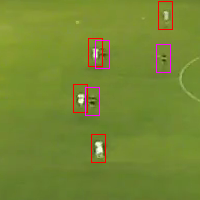
\includegraphics[width=1.4in]{./images/cropped_rendered002.png}
      \centering
      \footnotesize
      \textbf{(a)} Cuadro 2
    \end{minipage}
    \hspace{-0.3cm}
    \begin{minipage}[t]{.25\textwidth}
      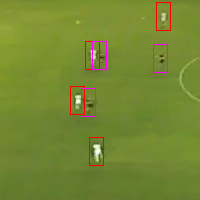
\includegraphics[width=1.4in]{./images/cropped_rendered007.png}
      \centering
      \footnotesize
      \textbf{(b)} Cuadro 12
    \end{minipage}
    \hspace{-0.3cm}
    \begin{minipage}[t]{.25\textwidth}
      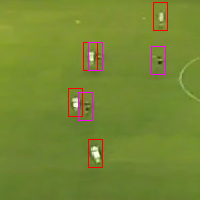
\includegraphics[width=1.4in]{./images/cropped_rendered012.png}
      \centering
      \footnotesize
      \textbf{(c)} Cuadro 14
    \end{minipage}
    \hspace{-0.3cm}
    \begin{minipage}[t]{.25\textwidth}
      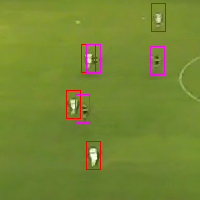
\includegraphics[width=1.4in]{./images/cropped_rendered017.png}
      \centering
      \footnotesize
      \textbf{(d)} Cuadro 17
    \end{minipage}
    %% NASTY hack to make refernce work with figures and subfigures, put \label inside \caption env, little bird told me
    \caption{Seguimiento de los jugadores en un video real mediante el algoritmo de contornos activos modificado.
    \label{fig:boca-activeContour}
    }
\end{figure}

Como se puede observar en la Figura \ref{fig:happy-occluded-activeContour}, el
algoritmo propuesto en este trabajo logra seguir con éxito a los objetos de
interés en el video sintético. Además, también se obtiene un resultado positivo
en el video real en la situación en que IFTrace pierde al jugador, como puede
observarse en la Figura \ref{fig:boca-activeContour}.

\subsection{Evaluación de Comportamiento}

Otro punto importante de comparación entre los dos algoritmos es su tiempo de
ejecución, es decir el tiempo que tarda en llevar a cabo su trabajo.  De
acuerdo a las mediciones realizadas con un video real de un partido de fútbol,
siguiendo a un solo jugador, el tiempo promedio que tarda IFTrace por cuadro es
6.962 segundos, mientras que el algoritmo implementado tiene un tiempo promedio
de 0.712 segundos. Se puede observar que se encuentra un orden magnitud por
debajo de IFTrace, incluso antes de realizar optimizaciones.
%% 6.9628571428571435 si quieren los decimales

Cabe destacar que ambos algoritmos podrían verse beneficiados de ciertas
optimizaciones, como ser por ejemplo la programación en GPU y la reducción de
operaciones de \textit{Input/Output} al almacenamiento secundario (disco duro).



\newpage

\chapter{Conclusiones}
\label{chap-conclusion}

Como se explica en la Capítulo \ref{chap-problems}, el problema en cuestión
tiene una gran complejidad, y ha sido objeto de interés y de estudio con
anterioridad. Se han dedicado muchos recursos y esfuerzo en la búsqueda de una
solución.

Teniendo en cuenta las numerosas y complejas dificultades, sumadas a las
restricciones del problema, se puede concluir que la solución propuesta en este
trabajo realiza un buen trabajo en el seguimiento de los jugadores en los
videos de fútbol. Resulta díficil obtener mejores resultados con los recursos
disponibles y las restricciones planteadas. Puede observarse como la solución
propuesta resulta flexible y capaz de recuperarse de forma semi-supervisada,
algo que otras técnicas complejas y robustas no contemplan, como por ejemplo la
técnica de \textit{IFTrace}.

%%TODO podemos decir que el material era malo? Y que era dificil
%% conseguir material de las mismas caracteristicas??

\section{Trabajo Futuro}

Queda como posible investigación futura la utilización de otras características
para representar a los objetos, como podrían ser otros espacios de colores, o
el uso de descriptores de texturas.

Cabe destacar que trabajos futuros se verían muy beneficiados de contar con más
material y de mejor calidad. Lo ideal sería poder escoger la ubicación de la
cámara de modo de utilizar eficientemente todo el cuadro de la imagen para la
cancha, y contar con cámaras de mayor resolución.

\subsection{Mejoras de performance}

Uno de los objetivos de investigación de este trabajo es lograr un seguimiento en
tiempo real, es decir procesar por lo menos 24 cuadros por segundo. La implementación
de referencia no cumple con este objetivo, pero tiene mucho lugar a optimización. 
Por ejemplo, El trabajo de preprocesamiento de un cuadro y de aplicación de Contornos
Activos puede distribuirse en 2 computadoras distintas. Esto permite tener una menor
latencia entre cuadro y cuadro, y podria duplicar la velocidad percibida. 

Existe tambien lugar a optimización en Contornos Activos. El algoritmo original no
esta diseñado para seguir 24 contornos en tiempo real. La implementación procesa
cada contorno de manera secuencial, desperdiciando la capacidad de multiprocesamiento
de las computadoras modernas. Se podria adaptar el algoritmo para aprovechar esta
capacidad y mejorar el tiempo de ejecución notablemente.

%- Mal material, imposible agarrar la pelota y difícil los jugadores
%- Resultados aceptables


\printbibliography

\newpage
\appendix
\chapter{Capturas de Pantalla de Aplicación}

\begin{figure}[H]
  \centering
  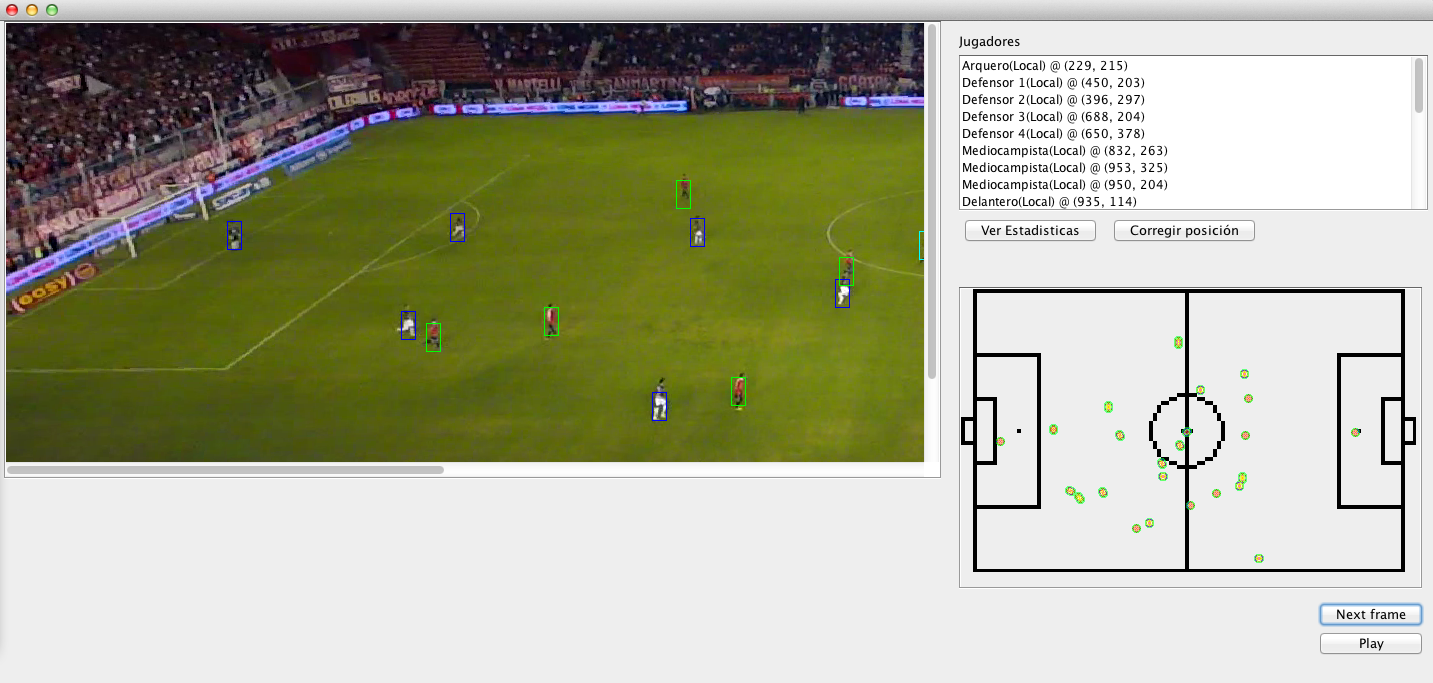
\includegraphics[width=\linewidth]{./images/Screen-Indep.png}
  \caption{Captura de pantalla utilizando el video de Independiente}
\end{figure}


\end{document}
